%\documentclass[10pt]{iopart}
\documentclass{article}
\usepackage{geometry}
\usepackage[nottoc]{tocbibind}
\usepackage{graphicx}
\usepackage{subfig}
\usepackage{amssymb}
\usepackage{amsmath}
\usepackage{amsthm}
\usepackage{slashed}
\usepackage{bm}
\usepackage{hyperref}
\usepackage{listings}
\usepackage[percent]{overpic}
\usepackage{cite}
\usepackage{braket}
\usepackage{yfonts}
\usepackage{subfig}
%\usepackage{axodraw4j} %for Feynman diagrams
\usepackage{braket}
%Uncomment next line if AMS fonts required
%\usepackage{iopams}
\numberwithin{equation}{section} %allows numbering of equations to include section number
\usepackage[utf8x]{inputenc}
\geometry{a4paper, total={6in, 8in}}

\allowdisplaybreaks

\begin{document}


\begin{titlepage}
\begin{center}
\vspace*{1cm}
Mathematical Tripos Part III\\Essay
\vspace{0.5cm}

{\LARGE \textbf{Anomalous Muon Magnetic Moment \\and Lattice QCD}}
\vspace{3cm}

%Andrew Zhen Ning Yong\\
%Supervisor: Dr Christopher Thomas\\
\vspace{1cm}
\vspace{7cm}
Department of Applied Mathematics and Theoretical Physics\\
University of Cambridge\\
%4\textsuperscript{th} March 2018

%\begin{abstract}\end{abstract}

\end{center}
\end{titlepage}

\newcommand{\amu}{$a_\mu$ }

\tableofcontents

\newpage

\section{Introduction}\label{intro}
The anomalous muon magnetic moment, $a_\mu$, is an additional contribution to the lepton's magnetic moment due to loop corrections. This deviation from the magnetic moment predicted by Dirac's theory can be defined as\cite{lehnerg2}

\begin{equation}
a_\mu = \frac{g-2}{2},
\label{amu}
\end{equation}

\noindent where g is the Land\'e g-factor.  

The anomalous muon magnetic moment receives contributions from all sectors of the Standard Model. To make this point manifest, we can split \amu based on the contributing sectors\cite{hoecker},

\begin{equation}
a^{\mathrm{SM}}_\mu= a_\mu^{\mathrm{QED}} + a_\mu^{\mathrm{EW}} + a_\mu^{\mathrm{had}},
\label{asm}
\end{equation}

\noindent corresponding to radiative corrections due to virtual leptons and photons, gauge bosons and hadrons respectively. As a consequence, performing a precision measurement on \amu allows us to probe for new physics since any coupling of the muon to undiscovered particles, be it through Standard Model interactions or beyond, will contribute to the anomalous magnetic moment\cite{fermilab}. Thus, any discrepancies found between the measured \amu and the Standard Model prediction could provide hints of interactions that are unaccounted for in the theory. 

In this literature review, we will first acquaint ourselves with the origin of the anomalous magnetic muon. This is followed by a review of the measurements made in the Brookhaven National Laboratory (BNL) during the E821 experiment. The main section of the review will be devoted to studying the methods used in evaluating hadronic contributions to the anomalous muon magnetic moment. The  low energy  regime of Quantum Chromodynamics (QCD) is non-perturbative. Thus, we rely on ever-improving numerical techniques developed in the vibrant field of Lattice Quantum Chromodynamics.

\section{g-2: A Brief History}\label{hist}

Here the origin of the anomalous magnetic moment is presented in a brief historical narration. A more detailed account of the history on g-2 can be found in the review by Miller, de Rafael and Roberts\cite{millerg2}.

Experiments such as those performed by Stern and Gerlach in 1922 and Phipps and Taylor in 1927 revealed that the magnetic moment of the atoms in the presence of a non-uniform magnetic field are split into two bands, representing two discrete values for the z-component of the magnetic moment\cite{phipps}. The interpretation given by Uhlenbeck and Goudsmit was that the unpaired electron in both the silver atoms (Stern \& Gerlach) and the hydrogen beam (Phipps \& Taylor) has an intrinsic angular momentum built in. This angular momentum, now known as the \textit{spin} angular momentum, is quantum in nature and is responsible for the discrete values of the magnetic moment.

The magnetic moment, $\vec{\mu}$, of a charged particle has the following form\cite{hoecker}

\begin{equation}
\vec{\mu}=g\frac{q}{2m}\vec{S},
\label{magnetic moment}
\end{equation}

\noindent where $q$ and $m$ are the charge and mass of the particle respectively, $g$ is the Land\'e g-factor and $\vec{S}$ is the spin angular momentum. The two bands observed in the experiments correspond to the fact that the electrons are spin-1/2 particles. Thus, the z-component of the spin may take on two discrete values, $s_z=\pm \hbar/2$. Using the fact that the experiments measured the z-component of the magnetic moment to be one Bohr magneton, $e\hbar/2m_e$, the Land\'e g-factor is deduced to be $g=2$.

In fact, the value of the g-factor was also predicted from Dirac's wave equation for relativistic electrons in 1928. The Klein-Gordon equation of the electron can be manipulated\cite{zee} to yield 

\begin{equation}
\left(-2im\frac{\partial}{\partial t} - \nabla^2 - e\vec{B}\cdot (\vec{L} + 2 \vec{S}) \right)\psi=0. 
\label{KGeq for rel e}
\end{equation}

\noindent The g-factors for the orbital and spin angular momentum are the coefficients that couple to their respective operators, where we see that g=2 emerges naturally for the spin of an electron.

However, in 1947, experimental evidence indicated that the splitting due to the hyperfine structure of the hydrogen is larger than that predicted from the Dirac theory\cite{lehnerg2}. The insight provided by Schwinger is that this is due to loop corrections to the magnetic moment, where the electron radiates virtual particles in the presence of a magnetic field. To account for this discrepancy, we can split the magnetic moment into two pieces,

\begin{equation}
\mu = (1+a)\frac{q\hbar}{2m},
\end{equation}

\noindent where the first piece corresponds to the prediction from Dirac's theory and the second piece, $a$, is defined in Equation \ref{amu}. One can then predict $a$ by computing loop corrections. Although this was originally proposed to resolve the disagreement between measurement and prediction of the electron magnetic moment, we know now that this anomaly is present in both muons and tauons as well. However, for the remainder of this review we will concern ourselves with \amu and the justification for this will be provided in the beginning paragraph of \S\ref{th}.






\section{Experimental Measurements}\label{exp}
The value for \amu has been measured to ever increasing precision in the last 50 years, with the first precision measurement made during the CERN I experiment in 1961\cite{fermilab} to the more recent E929 experiment in Fermilab that begun taking data in 2017. Since the CERN III experiment in 1974, the general setup for the muon g-2 experiments has been the same, with improvements introduced by the team in Brookhaven National Laboratory (BNL) in the subsequent decades. The discussion below follows the setup from the E821 experiment from BNL\cite{bnl}.

A beam of protons is accelerated to hit a target. These collisions produce pions, which are steered into a long beamline where they decay into muons and neutrinos. For a process such as $\pi^+ \rightarrow \mu^+\nu_\mu$, the high energy muons are selected. This selection criteria corresponds to muons which decay in the direction of the original pion's trajcetory. The parity violating nature of the weak interaction means that these muons are exclusively left-handed\cite{sm}. The polarised beam are then injected into the muon storage ring with cyclotron frequency, $\omega_c$. They remain in orbit under a uniform magnetic field, $B$, where the spin of the muons precesses with frequency, $\omega_s$.

By measuring the difference between the cyclotron and spin precession frequency, the anomalous muon magnetic moment can be quantified as

\begin{equation}
\vec{\omega}_a \equiv \vec{\omega}_s-\vec{\omega}_c = \frac{e}{m}\left( a_\mu \vec{B}-(a_\mu-\frac{1}{\gamma^2-1})\frac{\vec{\beta}\times\vec{E}}{c}\right),
\label{omega_a}
\end{equation} 

\noindent where $e$ and $m$ are the charge and mass of the muon respectively, $\vec{B}$ is the magnetic field perpendicular to the plane of the muon orbit, $\vec{E}$ is the quadrupole electric field and $\vec{\beta}$ and $\gamma$ are the usual relativistic beta and Lorentz factor of the muon respectively. The speed of light $c$ was also included to give $\omega_a$ the right dimension. By selecting muons with the ``magic'' momentum, $p_\mu=3.094$GeV/c corresponding to a Lorentz factor of $\gamma\approx 29.3$, to enter the muon storage ring, the electric quadrupole term in Equation \ref{omega_a} vanishes. The determination of \amu amounts to precise measurements of the magnetic field $B$ and the precession frequency, $\omega_a$ as the following form suggests

\begin{equation}
\omega_a=a_\mu\frac{eB}{m}.
\label{omega_a1}
\end{equation}

The magnetic field can be measured in terms of the NMR frequency of the free proton, $\omega_p$. Thus, Equation \ref{omega_a1} can be rewritten as

\begin{equation}
\begin{split}
a_\mu &= \frac{\omega_a}{\omega_L-\omega_a},\\
&= \frac{\omega_a/\omega_p}{\omega_L/\omega_p-\omega_a/\omega_p},\\
\Rightarrow a_\mu&= \frac{\mathrm{R}}{\lambda-\mathrm{R}},
\end{split}
\end{equation}

\noindent where $\omega_L$ is the Larmor precession of the muon. The muon-to-proton magnetic moment ratio, $\lambda$, is determined from the measurement of the Zeeman ground state hyperfine transition of the muonium\cite{muon_hyperfine}. Thus, the BNL experiment E821 was tasked to measure the ratio R in order to determine the value of \amu.

From the precision measurements done by W. Liu et al.\cite{muon_hyperfine}, the muon-to-proton ratio was determined to be, $\lambda =3.183 345 13(39)$, where te uncertainty quoted is due to statistical errors. The report compiled by G. W. Bennet \textit{et al.}\cite{bnl} studied the experimental measurements that were conducted through the years between 1999 to 2001. In total, there were two R ratios for $\mu^+$ and one for $\mu^-$, taken from the R99, R00, R01 experiments. By assuming CPT invariance, the average of the three R ratios are

\begin{equation}
\mathrm{R}_\mu^{\mathrm{E821}} = 0.003 707 206 4(2 0).
\end{equation}

\noindent This gives the experimental value of the anomalous magnetic moment\cite{millerg2}

\begin{equation}
a_\mu^{\mathrm{E821}} = 11 659 208.0(5.4)(3.3) \times 10^{-10},
\label{a_mu exp}
\end{equation}

\noindent where the statistical and systematic uncertainties are given respectively. With the R01 period finished, the Brookhaven muon g-2 experiments are now formally completed. As mentioned in the opening paragraph of this section, the E929 experiment at Fermilab will aim to further reduce the uncertainties of the \amu measurement, with the goal of improving the precision by four-fold\cite{fermilab}.



%The combined uncertainty works out to be 0.54ppm. This demonstrates a 14-fold improvement compared to the uncertainties in the experiments performed at CERN.



\section{Theory - Standard Model Predictions}\label{th}

All known charged leptons possess an anomalous magnetic moment. As of 2007, the experimental uncertainty of the muon anomalous magnetic moment is $\pm0.05$ppm. This is about 770 times larger than that of the electron anomalous magnetic moment\cite{millerg2}. Despite the greater uncertainty, there is a strong theoretical motivation for using the muon as the main probe for new physics. Namely, it is more sensitive to non-QED contributions than the electron. The contribution to the anomalous magnetic moment due to a massive virtual particle, $M_X$, scales as $(m/M_X)^2$, where $m$ is the mass of the charged lepton. This means that $a_\mu$ is $(m_\mu/m_e)^2\approx 40000$ more sensitive to such contributions than that of $a_e$\cite{fermilab}. In principle, this would make $a_\tau$ the best probe for new physics from the lepton sector. However, due to its much shorter lifetime\footnote{For reference, $\tau_\mu=(2.1969811 \pm 0.0000022)×10^{-6}$s and $\tau_\tau=(290.3 \pm 0.5) × 10^{-15}$s\cite{pdg}.}, this poses a formidable challenge for precision measurements in experiments\cite{fermilab}.

Since any discrepancy between theoretical prediction and experimental measurement can hint at new physics currently unaccounted for by the Standard Model, it is therefore in our best interest to produce $a_\mu^\mathrm{SM}$ to a precision standard that matches that of experiments. In this section, we will discuss the progress in calculating $a_\mu^\mathrm{SM}$. We begin by briefly reviewing the successes in obtaining the QED and electroweak contributions. The remainder of this ltierature review will be dedicated to confronting the non-perturbative nature of hadronic contributions.

\subsection{QED Contributions}

In discussing contributions due to QED processes, we will mainly be following the review produced by Jegerlehner and Nyffeler\cite{lehnerg2} and the results of Aoyama \textit{et al.}\cite{aoyama} A sample of Feynman diagrams involving QED interactions can be found in Figure\ref{qedfeynman}.

\begin{figure}[t]
    \centering
    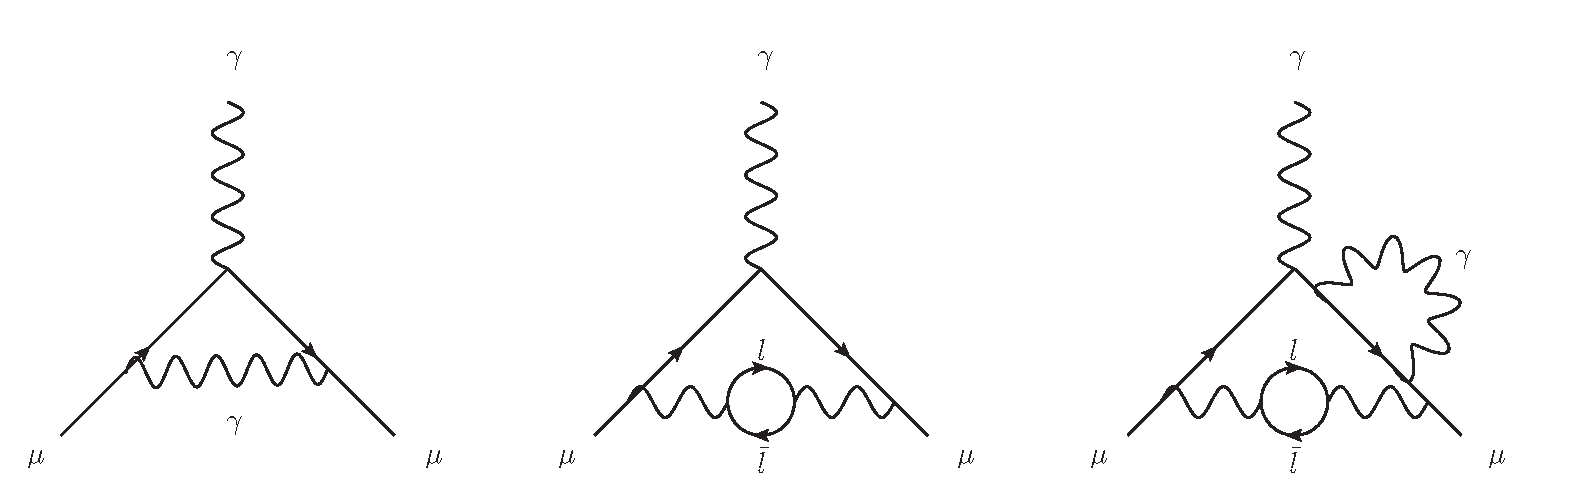
\includegraphics[width=12cm]{qed.eps}%
    \caption{Sample Feynman diagrams depicting QED contributions to the muon anomalous magnetic moment. \textbf{Left}: lowest order universal term - the famous Schwinger term. \textbf{Centre}: one of 9 second order mass dependent term. \textbf{Right}: one of 72 third order mass dependent term. Note that mass dependent terms can become universal terms when $l=\mu$.}%
    \label{qedfeynman}%
\end{figure}

Historically, contributions from Quantum Electrodynamics to the anomalous magnetic moment of leptons were the first to be accounted for. The famous work by Schwinger\cite{schwinger} determined the first order QED contribution to be $\alpha/2\pi$, where $\alpha$ is the fine structure constant. In principle, the smallness of $\alpha$ allows one to compute arbitrarily high order contributions analytically. Unfortunately, in practice, the number of Feynman diagrams become unmanageable and the amplitudes increasingly difficult to compute. Instead, numerical integrations are employed, for example, from four-loop diagrams onwards\cite{aoyama}.

To compute the QED contributions to $a_\mu^\mathrm{SM}$, we write the QED sector as

\begin{equation}
a_\mu^\mathrm{QED} = \sum_{n=1}^\infty \left(\frac{\alpha}{\pi}\right)^n a_\mu^{(2n)},
\label{aqed}
\end{equation}

\noindent where $n$ refers to the $n$-loop correction. We can further organise the terms of $a_\mu^{(2n)}$ as

\begin{equation}
a_\mu^{(2n)} = A_1^{(2n)} + A_2^{(2n)}\left(\frac{m_\mu}{m_e}\right) + A_2^{(2n)}\left(\frac{m_\mu}{m_\tau}\right) + A_3^{(2n)}\left(\frac{m_\mu}{m_e}, \frac{m_\mu}{m_\tau}\right),
\end{equation}

\noindent where $A_1^{(2n)}$ are the mass independent (universal) contributions and $A_2^{(2n)}$ are the mass dependent terms. We note that for $n=2,3$, the contributions are known analytically. For $n\gtrsim 4$, Aoyama \textit{et al.} resorted to numerical integration, as stated above. 

It is clear from Equation \ref{aqed} that a precise prediction of $a_\mu^\mathrm{QED}$ requires precise knowledge of the lepton mass ratios and the fine structure constant. For the former, Aoyama referred to the values provided by CODATA\cite{codata}, namely $m_\mu /m_e = 206.7682843(52)$ and $m_\mu /m_\tau = 5.94649(54) \times 10^{-2}$. As for the latter, two different approaches were used to obtain $\alpha$: one by the precisely measured Rydberg constant (denoted Rb below) and the other via the anomalous magnetic moment of the electron. 

Below, we quote the QED contributions to $a_\mu^\mathrm{SM}$ up to the $n=5$-loop correction, using two different determinations of $\alpha$:

\begin{equation}
\begin{split}
a_\mu^\mathrm{QED}(\mathrm{Rb}) &= 116584718951(9)(19)(7)(77)\times 10^{-14},\\
a_\mu^\mathrm{QED}(a_e) &= 116584718846(9)(19)(7)(30)\times 10^{-14}
\end{split}
\label{aqed_final}
\end{equation}

\noindent where the uncertainties are due to the lepton mass ratios, the 4- and 5-loop correction terms and $\alpha_e$ respectively.

As we will see in subsequent sections, $a_\mu^\mathrm{QED}$  contributes the most to $a_\mu^\mathrm{SM}$ out of all the other terms in Equation \ref{asm}. Thus, it remains an important effort to further reduce the uncertainties in Equation \ref{aqed_final} and to strive for higher loop terms.



%
%The QED contributions come from photonic and leptonic loops. Starting with the famous Schwinger result, $\alpha/2\pi$\cite{hoecker}, the muons can emit virtual photons which are reabsorbed again at a later time. Alternatively, the photons can also undergo pair-production, producing a lepton-antilepton pair. We see that the stark difference between these two types of loop corrections is the presence of mass terms. Folloing this line of reasoning, let us further break the QED contribution to \amu as\cite{qedg2}
%
%\begin{equation}
%\begin{split}
%a_\mu^{\mathrm{QED}}&=\sum_{n=1}^\infty \left(\frac{\alpha}{\pi}\right)^nA^{(2n)},\\
%A^{(2n)} =& A^{(2n)}_1 + A^{(2n)}_2\left(\frac{m_\mu}{m_e}\right) + A^{(2n)}_2\left(\frac{m_\mu}{m_\tau}\right) + A^{(2n)}_3\left(\frac{m_\mu}{m_e},\frac{m_\mu}{m_\tau}\right),
%\end{split}
%\label{aqed}
%\end{equation}
%
%\noindent where $\alpha$ is the fine structure constant, $A^{(2n)}_1$ represents the mass independent contributions called the \textit{universal} term and $A^{(2n)}_2$ and $A^{(2n)}_3$ are the mass-dependent terms. 
%
%Since both $A_2$ and $A_3$ are functions of mass ratios, it is now clear that $a_e$ would indeed receive a smaller QED contribution due to higher mass suppressions from the second and third generation leptons as compared to $a_\mu$.
%
%%These leptonic contributions would require the photon vacuum polarisation tensor, $\Pi_{\mu\nu}$. 



\subsection{Electroweak Contributions}

In this section, we will follow the progress made by Gnendiger \textit{et al.}\cite{gnendiger}. For details regarding the parametrisation used in determining the W mass, and subsequently $\alpha_\mu^\mathrm{EW}$, we refer to the 2012 particle physics review\cite{particle_review} used in Gnendiger's paper.

After QED processes, the next dominant contribution comes from the electroweak sector. Even so, we see that there exists strong suppression factors of at least $m_\mu^2/ M_W^2\approx 4\times 10^{-9}$\cite{hoecker}, owing to the massive gause bosons involved in the processes. According to Gnendiger\cite{gnendiger}, we can organise the electroweak contributions based on its order, that is

\begin{equation}
\alpha_\mu^\mathrm{EW} = \alpha_\mu^\mathrm{EW(1)}+\alpha_{\mu,\,b}^\mathrm{EW(2)}+\alpha_{\mu,\,f}^\mathrm{EW(2)} + \mathcal{O}(\alpha^{(3)}),
\end{equation}

\noindent where the bracketed numbers indicate the order in perturbation, the subscripts $b$ and $f$ represent bosonic and fermionic contributions respectively, as represented in Figure \ref{ewfeynman}. The higher, three-loop order as indicated by $\mathcal{O}(\alpha^{(0)}$, although dependent on the parametrisation used, is nonetheless heavily suppressed, of the order $\sim 0.4\times 10^{-11}$\cite{gnendiger}. As such, its contribution to $\alpha_\mu^\mathrm{EW}$ is negligible.

\begin{figure}[t]
    \centering
    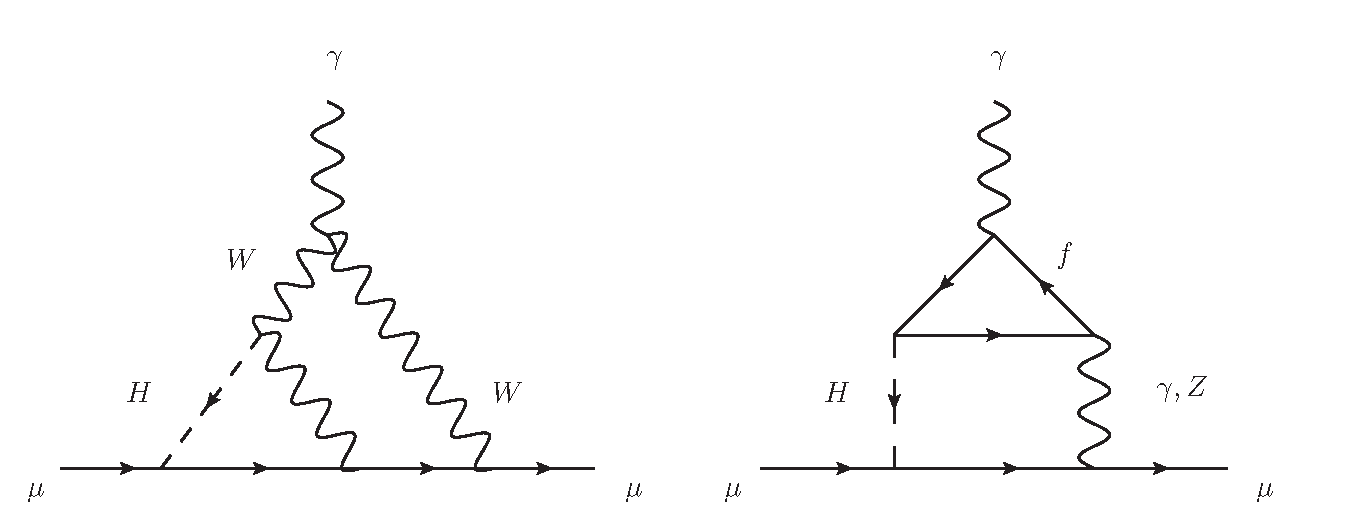
\includegraphics[width=12cm]{ew1.eps}%
    \caption{Feynman diagrams depicting second order electroweak contributions to the muon anomalous magnetic moment. \textbf{Left}: Higgs-dependent bosonic interaction. \textbf{Right}: triangular loop fermionic interaction.}%
    \label{ewfeynman}%
\end{figure}

The first order contribution can be expressed as

\begin{equation}
\alpha_\mu^\mathrm{EW(1)} = \frac{G_F}{\sqrt{8}}\frac{m_\mu^2}{8\pi^2}\left(\frac{5}{3} + \frac{1}{3}(1-s_W^2)\right)+\mathcal{O}\left(\frac{m_\mu^2}{M_H^2}\right) +\mathcal{O}\left(\frac{m_\mu^2}{M_W^2}\right),
\label{ew1}
\end{equation}

\noindent where $G_F$ is the Fermi constant and $s_W^2=1-(M_W/M_Z)^2$ is the weak mixing angle squared and $m_\mu, M_W, M_Z, M_H$ are the muon, W, Z and Higgs boson mass respectively. The first term in Equation \ref{ew1} is the dominant factor since the second and third is heavily suppressed by the gauge bosons' mass squared, this gives us the first electroweak contribution of\cite{gnendiger}

\begin{equation}
\alpha_\mu^\mathrm{EW(1)} = (194.80\pm 0.01)\times 10^{-11},
\label{ew1val}
\end{equation}

\noindent where the uncertainty is due input parameters, namely, the mass of the W boson. 

Since the determination of the Higgs boson mass, $M_H$ in 2012, we can now compute the second order contributions. The bosonic part gives

\begin{equation}
\alpha_{\mu, \, b}^\mathrm{EW(2)} = (-19.97 \pm 0.03)\times 10^{-11},
\end{equation}

\noindent where the uncertainty is due to the determination of the Higgs mass. To that end,  Gnendiger \textit{et al.} have chosen to use the average central value from CMS and ATLAS experiments, giving $M_H =(125.6\pm 1.5)$GeV.

On the other hand, the right diagram in Figure \ref{ewfeynman} receives contributions from lepton and quark loops. It is to no surprise that this value has uncertainties dominated by quark interactions. Here, we give the value of $\alpha_\mu^\mathrm{EW(2)}$, determined from $e, \mu, u, c , d , s$ interactions

\begin{equation}
\alpha_\mu^\mathrm{EW(2)} = (-6.91\pm 0.20\pm 0.30)\times 10^{-11},
\end{equation}

\noindent where the first and second uncertainties are due to first and second generation quark interactions respectively. Neglecting the strongly suppressed three-loop contribution of order $\mathcal{O}(10^{-12})$\cite{hoecker}, this gives us a total of

\begin{equation}
\alpha_\mu^\mathrm{EW} = (153.6\pm 1.0)\times 10^{-11},
\end{equation}

\noindent where the uncertainty is due to hadronic (quark and gluon) loop as seen in Figure \ref{ewfeynman}\cite{hoecker}.


\subsection{Hadronic Contributions - Preamble}

Difficulties arise when we evaluate $a_\mu^\mathrm{had}$ in the low energy regime. This is because the running strong coupling constant, $\alpha_s$, becomes large around $E\lesssim2$GeV\cite{lehnerg2} and we are forced to abandon our perturbative methods used in evaluating the QED and electroweak contributions. Instead, we will explore the role of lattice QCD in calculating $a_\mu^\mathrm{had}$. 

First, we will briefly illustrate the idea of computing quantum field theoretic observables on the lattice. To that end, we will follow the setup from Gattringer and Lang\cite{lattice}. This amounts to a simple principle of discretising spacetime. We can do so by replacing continuous space by a finite 3D lattice, $\Lambda_3$. Given a smooth variable, $\vec{x}\in\mathbb{R}^3$, we have

\begin{equation}
\vec{x} \rightarrow a \vec{n}, \quad \mathrm{with } \, \vec{n} = \begin{pmatrix}
n_1 \\ n_2 \\ n_3
\end{pmatrix},
\end{equation}

\noindent where $a$ is a constant known as the lattice spacing and $n_i\in\mathbb{Z}$ for $i=1,2,3$. We see that $\vec{n}$ is now a lattice vector that moves us from one lattice site to another. 

Similarly, fields which are originally functions of continuous spatial variable are now functions of coordinate vector of discrete spacing. For an arbitrary field operator, $\phi(\vec{x})$, we promote it to $\phi(\vec{x}) \rightarrow \phi(\vec{n})$. The generalisation to 4D spacetime is thus straightforward.

The lattice is to be implemented as an environment for numerical simulations. Thus, computing resources become one of the limiting factors. Since the lattice cannot span to infinity, we must impose boundary conditions. A suitable candidate would be periodic boundaries:

\begin{equation}
n_j=N \rightarrow n_j=0,
\end{equation}

\noindent for $j=1,2,3$. This means that for a lattice of length $N\cdot a$, where $N\in\mathbb{Z}$, we consider the coordinate $n_j=N$ to be equivalent to the origin.

We need to transfer our knowledge of calculus onto the lattice as well. To that end, for a derivative such as $\nabla\phi$, we can approximate it as

\begin{equation}
\partial_j\phi(\vec{x}) \approx \frac{\phi(\vec{x}+\vec{j})-\phi(\vec{x}-\vec{j})}{2a} + \mathcal{O}(a^2),
\label{lattice derivative}
\end{equation}

\noindent where $\vec{j}$ is another lattice vector that characterises the deviation from $\vec{n}$. The additional factor of 1/2 in Equation \ref{lattice derivative} is to account for averaging the deviation from $\vec{n}$. Similarly, for an integral over space, we can discretise it as such

\begin{equation}
\int d^3x \rightarrow a^3\sum_{\vec{n}\in\Lambda_3},
\label{lattice integral}
\end{equation}

\noindent which makes sense since we are now summing over the values associated to each discrete lattice site. It is easy to confirm the validity of these discretisations as we can always retrieve the contiuum expressions by taking the limit of $a\rightarrow 0$ in Equation \ref{lattice derivative} and \ref{lattice integral}. For further details regarding the lattice formalism, we refer to the textbook by Gattringer and Lang\cite{lattice}.

In the following, we will explore how the implementation of the lattice can aide us in computing $a_\mu^\mathrm{SM}$. As stated in \cite{lehnerg2}, the main theoretical uncertainty of $a_\mu$ is dominated by hadronic contributions. Namely, they come from two sources: the hadronic vacuum polarisation, $a_\mu^\mathrm{HVP}$, which comes in as second order electromagnetic corrections, and light-by-light scattering  processes, $a_\mu^\mathrm{HLbL}$, which is present at third order. These are shown in Figure \ref{hadfeynman}. For the most up-to-date progress on calculating the hadronic vacuum polarisation contributions, we will be following the review written by Della Morte \textit{et al.}\cite{dellamorte} in 2017. As for hadronic light-by-light processes, we will follow the progress made by Blum \textit{et al.}\cite{blum} in 2016. We will also follow the conventions set up in \cite{vector}: the Minkowski signature is (+ - - -); Euclidean momenta are denoted by upper case Latin letters ($K$, $Q$ etc.) and Minkowski momenta by lower case Latin letters ($k$, $q$ etc.).

At the end of the following two subsections, we will compare the lattice approaches with alternative methods that are currently being studied.


\begin{figure}[t]
    \centering
    \subfloat[]{{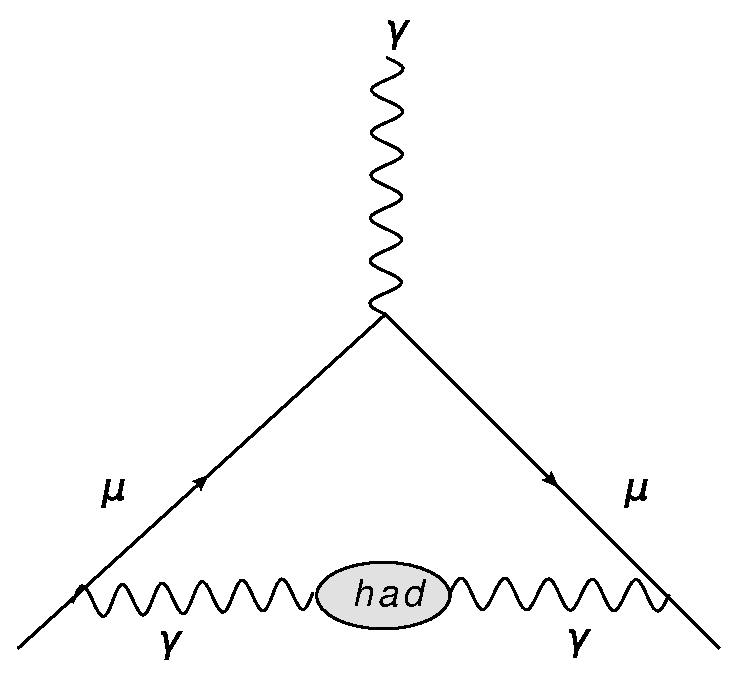
\includegraphics[width=5cm]{had.eps} }}%
    \qquad
    \subfloat[]{{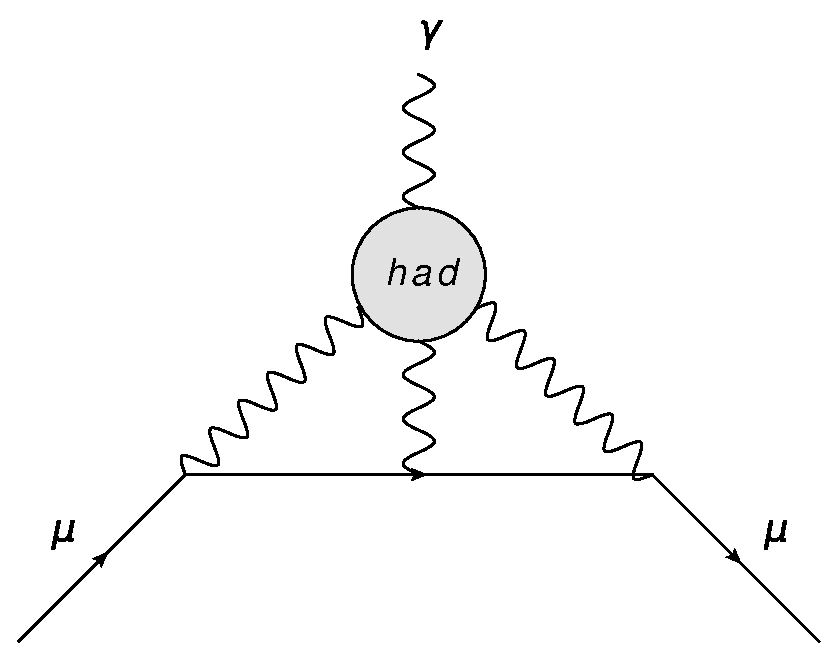
\includegraphics[width=5cm]{hadlbl.eps} }}%
    \caption{Feynman diagrams depicting hadronic contributions to the muon anomalous magnetic moment. \textbf{Left}: hadronic vacuum polarisation. \textbf{Right}: hadronic light-by-light scattering.}%
    \label{hadfeynman}%
\end{figure}


\subsection{Hadronic Vacuum Polarisation Contributions}\label{hvp}

Lattice calculations of $a_\mu^\mathrm{HVP}$ are done by evaluating a convolution integral over the Euclidean momenta $Q^2$. This integral (to be defined below) receives the largest contribution when $Q^2\approx m_\mu^2\approx 0.01\mathrm{GeV}^2$, which corresponds to 

\begin{equation}
\begin{split}
Q &= \frac{2\pi}{L},\\
L &= 2\pi Q^{-1},\\
&\approx 2\pi 10^{-1} \mathrm{GeV}^{-1} 0.2 \mathrm{GeV \, fm},\\
\Rightarrow L &\approx \mathcal{O}(10\mathrm{fm}), 
\end{split}
\end{equation}

\noindent where $L$ is the typical lattice length\cite{dellamorte}.

This low momentum falls below the smallest Fourier momentum in the typical lattice size. In particular, the problem lies in the ability to accurately determine the vacuum polarisation function, $\Pi(Q^2)$, and the additive renormalisation term, $\Pi(0)$. We will consider two solutions proposed in the paper by Della Morte \textit{et al.}\cite{dellamorte}: 


\begin{enumerate}
\item Evaluate $a_\mu^\mathrm{HVP}$ in time-momentum representation,
\item or represent the subtracted vacuum polarisation, $\Pi(Q^2)-\Pi(0)$, with Pad\'{e} approximants using time-moments,
\end{enumerate}

\noindent both of which we will discuss in detail below. 

We will begin by collecting the tools necessary for lattice QCD. First, we need the electromagnetic current. Recall the piece of the electroweak Lagrangian concerning the quark sector,

\begin{equation}
\mathcal{L}=i\bar{Q}_L\gamma^\mu D_\mu Q_L + i\bar{u}_R\gamma^\mu D_\mu u_R + i\bar{d}_R\gamma^\mu D_\mu d_R,
\label{ewqLagr}
\end{equation}

\noindent where we have used the following convention\cite{sm},

\begin{align*}
Q_L^i&=\begin{pmatrix}
\begin{pmatrix}
u\\d
\end{pmatrix}_L, & \begin{pmatrix}
c\\s
\end{pmatrix}_L, & \begin{pmatrix}
t\\b
\end{pmatrix}_L
\end{pmatrix},\\
u^i_R&=(u_R	,c_R,t_R),\\
d^i_R&=(d_R,s_R,b_R),
\tag{\refstepcounter{equation}\theequation}
\end{align*}

%\noindent to indicate that the left-handed quarks transform as a doublet and the right-handed quarks transform as a singlet under SU(2)$_\mathrm{L}$. The covariant derivative, $D_\mu$, contains gauge fields which can be rearranged to give charged, neutral and electromagnetic interaction terms. 

%The piece of the Lagrangian of interest to us is
%
%\begin{equation}
%\begin{split}
%\mathcal{L} &= ieA_\mu (C_1i\bar{Q}_L\gamma^\mu Q_L + iC_2\bar{u}_R\gamma^\mu u_R + iC_3\bar{d}_R\gamma^\mu d_R),\\
%C_1&\equiv \begin{pmatrix} Y_u+T^3 & 0 \\ 0 & Y_d+T^3
%\end{pmatrix}, \quad \mathrm{where \,} T^3=\frac{1}{2}\sigma^3,\\
%C_{2,3}&=Y_{2,3},
%\end{split}
%\label{emLagr}
%\end{equation}
%
%\noindent where $C_i$ are the charge matrices, $Y_i$ is the hypercharge associated to the quarks and $\sigma_3$ is the third Pauli matrix. We note the absence of $T^3$ in $C_2$ and $C_3$ is due to the fact that they transform as a singlet under SU(2)$_\mathrm{L}$. 

\noindent to indicate that the left-handed quarks transform as a doublet and the right-handed quarks transform as a singlet under SU(2)$_\mathrm{L}$. The covariant derivative, $D_\mu$, contains gauge fields which can be rearranged to give charged, neutral and electromagnetic interaction terms. 
Expanding the Lagrangian in Equation \ref{ewqLagr}, and inserting the appropriate hypercharges to give the correct quark charges, we find that it simplifies to

\begin{equation}
\mathcal{L}=-eA_\mu\left(\frac{2}{3}\bar{u}\gamma^\mu u -\frac{1}{3}\bar{d}\gamma^\mu d -\frac{1}{3}\bar{s}\gamma^\mu s + ...\right),
\end{equation}

\noindent where, for a given quark, $q=q_L + q_R$ and the ellipses denote the remaining heavier quarks. Using the fact that the above Lagrangian as a U(1)$_\mathrm{Y}$ symmetry, the electromagnetic current can be easily computed using Noether's theorem to give

\begin{equation}
J_\mathrm{EM}^\mu = \frac{2}{3}\bar{u}\gamma^\mu u -\frac{1}{3}\bar{d}\gamma^\mu d -\frac{1}{3}\bar{s}\gamma^\mu s + ...
\end{equation}

With the electromagnetic current, $J_\mathrm{EM}^\mu$, we can construct the vacuum polarisation tensor in Euclidean space, which is defined as

\begin{equation}
\Pi_{\mu\nu}(Q) = \int d^4x \, e^{iQx} \langle J_\mu(x) J_\nu(0)\rangle,
\end{equation}

\noindent where Q is the (Euclidean) momentum. 

It turns out that gauge invariance provides a strong constraint on the form $\Pi_{\mu\nu}(Q)$ can take. From the Ward-Takahashi identity\cite{zee}, we find that 

\begin{equation}
Q_\mu\Pi^{\mu\nu}(Q)=0,
\end{equation}

\noindent where as usual, the repeated Lorentz indices are contracted. Together with Lorentz invariance, the most general tensor structure for $\Pi_{\mu\nu}$ is

\begin{equation}
\Pi_{\mu\nu}(Q) =\left(Q_\mu Q_\nu - \delta_{\mu\nu}Q^2 \right)\Pi(Q^2),
\label{tensor structure}
\end{equation}

\noindent where $\delta_{\mu\nu}$ is the Euclidean metric and $\Pi(Q^2)$ is the vacuum polarisation function.

With the quantities defined above, we are now in the position to calculate the hadronic vacuum polrisation contribution to $a_\mu$, which is defined as 

\begin{equation}
a_\mu^\mathrm{HVP} = 4\alpha^2 \int_0^\infty dQ^2 \, K(Q^2;m_\mu^2) \left(\Pi(Q^2) - \Pi(0) \right),
\label{ahvp}
\end{equation}

\noindent where $\alpha$ is the electromagnetic coupling constant and $K(Q^2;m_\mu^2)$ is a kernel function. The kernel here plays the role of an integral transform, intended to map the original domain (Euclidean momenta squared) to a different domain, where the evaluation of the integral may be easier. 

In Equation \ref{ahvp}, we find that the integral makes a significant contribution when $Q^2\approx m_\mu^2\approx 0.01$GeV$^2$. As mentioned in the beginning paragrahs, the corresponding long wavelength regime is hard to evaluate on the lattice with available resources. Below, we will look at the solutions proposed by Della Morte\cite{dellamorte}.

\subsubsection{Time Momentum Representation}\label{tmr}

Previously we introduced a kernel function, $K(Q^2;m_\mu^2)$, into Equation \ref{ahvp}. It is precisely the mapping property of the kernel that we can exploit to circumvent the long wavelength problem. In this subsection, we will begin with the review on vector correlators by Bernecker \textit{et al.}\cite{vector}. First, a slight change of notation: in literature it is often convenient to express the subtracted vacuum polarisation function as

\begin{equation}
\hat{\Pi}(Q^2) = 4\pi^2(\Pi(Q^2) - \Pi(0)),
\end{equation}

\noindent where the $4\pi^2$ is present due to convention used. So Equation \ref{ahvp} is now 

\begin{equation}
a_\mu^\mathrm{HVP} = \left(\frac{\alpha}{\pi}\right)^2 \int_0^\infty dQ^2 \, K(Q^2;m_\mu^2) \,\hat{\Pi}(Q^2).
\end{equation}

In the time momentum representation, the subtracted vacuum polarisation, $\hat{\Pi}(Q^2)$, is proportional to the vector correlator, $G(x_0)$. This is a quantity that spatially sums the electromagnetic currents and it is defined as

\begin{equation}
G(t) = \int d^3x \, \langle J_z(t,\vec{x})J_z^\dag(0)\rangle,
\label{vector correlator}
\end{equation}

\noindent where in Euclidean space, the spatial current is antiHermitian, $j^\dag_z=-j_z$\cite{vector}. We recognise that Equation \ref{vector correlator} is equivalent to the inverse Fourier transform of the vacuum polarisation tensor. In particular, the z-z component,

\begin{equation}
\begin{split}
\Pi_{zz}(Q) &= \int dt\,d^3x \, \langle J_z(x) J_z(0)\rangle e^{i\omega t},\\
&= \int dt \, G(t) e^{i\omega t},\\
\Rightarrow G(t) &= \int \frac{d\omega}{2\pi} \Pi_{zz}(\omega,k^i=0)e^{-i\omega t}
\end{split}
\label{G and Pi}
\end{equation}

\noindent The tensor structure of $\Pi_{zz}$ follows from Equation \ref{tensor structure},

\begin{equation}
\begin{split}
\Pi_{zz}(Q) &=\left(Q_z Q_z - \delta_{zz}Q^2 \right)\Pi(Q^2),\\
\Pi_{zz}(\omega,k^i=0) &=\left(0 - \omega^2 - 0 \right)\Pi(\omega,k^i=0),\\
\Pi_{zz}(\omega) &= -\omega^2\Pi(\omega).
\end{split}
\label{pi zz}
\end{equation}

\noindent Comparing Equation \ref{pi zz} and \ref{G and Pi}, we see that 

\begin{equation}
\Pi(\omega^2)= -\frac{1}{\omega^2}\int dt \, G(t) e^{i\omega t}.
\label{hvp - correlator}
\end{equation}

We are interested in the infrared regime, where conventional lattice calculations face difficulties. Expanding the exponential as a power series, we have

\begin{align*}
\Pi(\omega^2)&= \frac{-1}{\omega^2}\int dt \, G(t) \sum_{n=0}^\infty \frac{(i\omega t)^n}{n!},\\
&= \frac{-1}{\omega^2}\int dt \, G(t) \left(1 +i\omega t+\frac{1}{2!}(i\omega t)^2 + \mathcal{O}(\omega^2) \right),\\
&= \frac{-1}{\omega^2} \left(\int dt \, G(t) + i\omega \int dt \, G(t)t-\frac{1}{2!}\omega^2 \int dt \, G(t)t^2 + \mathcal{O}(\omega^2) \right).
\tag{\refstepcounter{equation}\theequation}
\end{align*}

\noindent We note that the first integral on the final line vanishes as we can identify it as the quark number susceptibility of the vacuum. For the term linear in $t$, we note that $G(t)$ is an even function, so the integral of $G(t)$ with $t$ - an odd function - across the boundaries therefore also vanishes. Keeping the first term, the subtracted vacuum polarisation function is thus

\begin{equation}
\begin{split}
\Pi(\omega^2)-\Pi(0) &= \int^\infty_{-\infty} dt \, G(t) \left( \frac{e^{-i\omega t} - 1}{\omega^2} + \frac{t^2}{2}\right),\\
&=\frac{2}{\omega^2}\int^\infty_0dt \, G(t) \left( \frac{\omega^2t^2}{2}-(\mathrm{cos\,} \omega t- 1) \right),\\
\Pi(\omega^2)-\Pi(0) &=\frac{1}{\omega^2}\int^\infty_0dt \, G(t) \left( \omega^2t^2-4\mathrm{sin\,}^2 \frac{1}{2}\omega t \right),
\end{split}
\end{equation}

\noindent where in going to the second line, we applied Euler's formula and noted that the $i\, \mathrm{sin\,}\omega t$ term is an odd function and causes the integral to vanish; we also gain a factor of 2 from the symmetric integration boundaries and this is used in the trigonometric identity to get the sine squared term in the final line. Inserting a factor of $4\pi^2$, we arrive at the desired modified expression

\begin{equation}
\hat{\Pi}(\omega^2) = 4\pi^2\int^\infty_0 dt\, G(t) \left( t^2-\frac{4}{\omega^2}\,\sin^2\, \frac{1}{2}\omega t \right).
\end{equation}

Now, we may rewrite our expression for $a_\mu^\mathrm{HVP}$,

\begin{equation}
\begin{split}
a_\mu^\mathrm{HVP} &= \left(\frac{\alpha}{\pi}\right)^2 \int_0^\infty d\omega^2 \, K(\omega^2;m_\mu^2) \,\hat{\Pi}(\omega^2),\\
&= \left(\frac{\alpha}{\pi}\right)^2 4\pi^2  \int_0^\infty \frac{d\omega^2}{\omega^2} \, dt\, K(\omega^2;m_\mu^2) \,G(t) \left( \omega^2 t^2-4\,\sin^2\, \frac{1}{2}\omega t \right),
\end{split}
\end{equation}
\begin{equation}
\begin{split}
a_\mu^\mathrm{HVP}&= \left(\frac{\alpha}{\pi}\right)^2  \int_0^\infty dt\, \tilde{K}(t;m_\mu) \,G(t) ,\\
\mathrm{with}& \quad \tilde{K}(t;m_\mu) \equiv \tilde{f}(t) = 4\pi^2 \int_0^\infty \frac{d\omega^2}{\omega^2} \, K(\omega^2;m_\mu^2) \,\left( \omega^2t^2-4\,\sin^2\, \frac{1}{2}\omega t \right),
\end{split}
\label{amu}
\end{equation}

\noindent where $\tilde{K}(t;m_\mu)$ is the time-momentum representation of the original kernel.

In order to evaluate $a_\mu^\mathrm{HVP}$, we need the correct expression for $\tilde{K}(t;m_\mu)$. For the remainder of this subsection, we will refer to the derivation in \cite{dellamorte} for an expression that can be used on the lattice. Further, we will use $\tilde{K}(t;m_\mu)$ and $\tilde{f}(t)$ interchangeably and similarly for $K(\omega^2;m_\mu^2)$ and $f(\omega^2)$. 

Since $a_\mu^\mathrm{HVP}$  is a dimensionless unit, we can deduce that the mass dimensions of $\tilde{f}(t)$ is -2 since the integral measure $dt$ has mass dimensions -1 and the $G(t)$ term has 4 copies of Dirac fermions integrated over 3-space, giving mass dimensions $\frac{3}{2}\cdot 4 - 3 = 3$. Therefore, $m_\mu^2 \tilde{f}(t)$ would make a dimensionless function of $m_\mu t$. For the moment, we will set $m_\mu$ to unity. Once we obtain an expression for $\tilde{f}(t)$ we will restore the appropriate factors by dimensional analysis.

First, we note that $d\omega^2=2\omega d\omega$. The function $f(\omega^2)$, which is really $K(\omega^2;m_\mu^2)$ in disguise, then has the following form 

\begin{equation}
f(\omega^2) = \frac{1}{\omega\sqrt{\omega^2 + 4}} - 1 + \frac{\omega}{2}(\sqrt{\omega^2 + 4} - \omega),
\end{equation}

\noindent for $\omega>0$. We introduce an auxillary function, $\tilde{g}_\epsilon(t)$ as 

\begin{equation}
\tilde{g}_\epsilon(t) = \int^\infty_0 \frac{d\omega}{\sqrt{\omega^2 + \epsilon^2}} f(\omega^2 + \epsilon^2)\, \cos \omega t,
\label{aux func}
\end{equation}

\noindent where we have introduced an infrared regulator, $\epsilon$, to keep $\tilde{g}_\epsilon(t)$ from diverging in the long wavelength limit where $\omega\rightarrow 0$. Using the auxillary function, we can identify the following

\begin{equation}
\begin{split}
\int^\infty_0 \frac{d\omega}{\omega} f(\omega^2) &= \lim_{\epsilon\rightarrow 0} \tilde{g}_\epsilon(0),\\
\int^\infty_0 \frac{d\omega}{\omega} f(\omega^2)\omega^2 t^2 &= \lim_{\epsilon\rightarrow 0} (-1)\cdot\frac{\mathrm{d}^2\tilde{g}_\epsilon(t)}{\mathrm{d}t^2}\bigg\vert_{t=0} \cdot t^2,\\
&=\lim_{\epsilon\rightarrow 0} \, - \tilde{g}''_\epsilon(0)t^2,\\
\int^\infty_0 \frac{d\omega}{\omega} f(\omega^2)\,4 \sin^2 \frac{1}{2}\omega t &= \int^\infty_0 \frac{d\omega}{\omega} f(\omega^2)\,2(1- \cos\omega t) ,\\ 
&= \lim_{\epsilon\rightarrow 0}\, 2(\tilde{g}_\epsilon(0)-\tilde{g}_\epsilon(t)).
\end{split}
\end{equation}

\noindent Collecting all the terms together, we can re-express $\tilde{f}(t)$ as 

\begin{equation}
\begin{split}
8\pi^2\int^\infty_0 \frac{d\omega}{\omega}\, f(\omega^2)(\omega^2 t^2 - 4 \sin^2 \frac{1}{2}\omega t) &= 8\pi^2 \lim_{\epsilon\rightarrow 0} - \tilde{g}''_\epsilon(0)t^2 - 2(\tilde{g}_\epsilon(0)-\tilde{g}_\epsilon(t)),\\
\tilde{f}(t)&= 16\pi^2 \lim_{\epsilon\rightarrow 0}\tilde{g}_\epsilon(t) - \tilde{g}_\epsilon(0) - \frac{1}{2} \tilde{g}''_\epsilon(0)t^2.
\end{split}
\label{ftilde}
\end{equation}

Consider the $\tilde{g}_\epsilon(t)$ piece. When expanded out, it reads

%\begin{equation}
%\begin{split}
%\tilde{g}_\epsilon(t) &= \int^\infty_0 \frac{d\omega}{\sqrt{\omega^2+\epsilon^2}}\, \left( \frac{1}{\sqrt{\omega^2+\epsilon^2}\sqrt{\omega^2+\epsilon^2+4}} - 1 \right. \\
%&\quad \quad \quad + \left.\frac{\sqrt{\omega^2+\epsilon^2}}{2}(\sqrt{\omega^2+\epsilon^2+4} - \sqrt{\omega^2+\epsilon^2}) \right) \, \cos\omega t,\\
%&= \int^\infty_0 d\omega\, \frac{\cos\omega t}{(\omega^2+\epsilon^2)\sqrt{\omega^2+4}} - \frac{\cos \omega t}{\sqrt{\omega^2+\epsilon^2}}  \\
%&\quad \quad \quad \quad \quad \quad \quad \quad \quad \quad  + (\sqrt{\omega^2+4} - \sqrt{\omega^2+\epsilon^2}) \, \frac{\cos \omega t}{2},
%\end{split}
%\label{g_epsilon}
%\end{equation}

\begin{equation}
\tilde{g}_\epsilon(t) = \int^\infty_0 d\omega\, \frac{\cos\omega t}{(\omega^2+\epsilon^2)\sqrt{\omega^2+4}} - \frac{\cos \omega t}{\sqrt{\omega^2+\epsilon^2}} + (\sqrt{\omega^2+4} - \sqrt{\omega^2+\epsilon^2}) \, \frac{\cos \omega t}{2},
\label{g_epsilon}
\end{equation}

Let's focus on the first term in the integrand, that is

\begin{equation}
I(t) = \int^\infty_0 d\omega\, \frac{\cos \omega t}{(\omega^2+\epsilon^2)\sqrt{\omega^2+4}}.
\end{equation}

\noindent This integral is difficult to evaluate from brute force integration. Instead, we turn $I(t)$ into a differential equation that satisfies the following initial conditions

\begin{equation}
\begin{split}
I''(t) - \epsilon^2I(t) &= -K_0(2t),\\
I(0) = \frac{\pi}{4\epsilon} - \frac{1}{4} + \mathcal{O}(\epsilon) &\quad \quad I'(0) = 0,
\end{split}
\label{diff eq I}
\end{equation}

\noindent where $K_0(2t)$ is the modified Bessel function of the second kind\cite{bessel} and the primes indicate time derivatives as usual. For the inhomogenous case, we can express $K_0(2t)$ with an integral representation \cite{bessel},

%First, consider the homogenous case:
%
%\begin{equation}
%I_0''(t) - \epsilon^2I_0(t)=0
%\end{equation}
%
%\noindent We find that this is simply $I_0(t) = Ae^{\epsilon t} + Be^{-\epsilon t}$. 

\begin{equation}
K_0(t) = \int^\infty_1 du \, \frac{e^{-ut}}{\sqrt{u^2-1}}.
\end{equation}

%\noindent Rescaling $K_0(t)$ with $t\rightarrow 2t\,\, \mathrm{and\,}\, u \rightarrow \frac{1}{2}u$, we find
%
%\begin{equation}
%K_0(2t) = \int^\infty_2 du \, \frac{e^{-ut}}{\sqrt{u^2-4}}.
%\end{equation}

\noindent Rescaling $K_0(t)$ with $t\rightarrow 2t\,\, \mathrm{and\,}\, u \rightarrow \frac{1}{2}u$, we find the particular solution, $I_p(t)$, by taking the Laplace transform\cite{laplace},

\begin{equation}
I_p(t) = \int^\infty_0 \, du \, e^{-ut} \tilde{I}(u),
\end{equation}

\noindent and match $\tilde{I}(u)$ with $-K_0(2t)$. Doing so, we find that

\begin{equation}
I_p''(t) - \epsilon^2 I_p(t) = (u^2-\epsilon^2)\int^\infty_0 \, du \, e^{-ut} \tilde{I}(u).
\end{equation}

\noindent If we look up a table of integral transforms, for example see \cite{laplace}, we find that the explicit expression for $\tilde{I}(u)$ is

\begin{equation}
\tilde{I}(u) = -\frac{H(u-2)}{(u^2-\epsilon^2)\sqrt{u^2-4}},
\end{equation}

\noindent where $H(u-2)$ is the Heaviside step function. The particular solution is thus 

\begin{equation}
I_p(t) = \int^\infty_2 du \, \frac{e^{-ut}}{u^2\sqrt{u^2-4}},
\label{particular solution}
\end{equation}

\noindent where we allow $\epsilon\rightarrow 0$ as Equation \ref{particular solution} is a valid solution to the differential equation. We note that $I_p(0) = -\frac{1}{4}$ and $I'(0) = \frac{\pi}{4}$. Combining the particular solution with a general solution, $I_0(t)$, and taking into account the initial conditions, we find the exact expression

%\begin{equation}
%\begin{split}
%I_\epsilon(t) &= I_0(t) + I_p(t),\\
%\mathrm{using \,} \,I_\epsilon(0) &= \frac{\pi}{4\epsilon} - \frac{1}{4} + \mathcal{O}(\epsilon),\\ 
%\frac{\pi}{4\epsilon} - \frac{1}{4} _ \mathcal{O}(\epsilon) & = I_0(0)  -\frac{1}{4},\\
%\Rightarrow I_0(0)&= \frac{\pi}{4\epsilon},\\
%\mathrm{using \,} \,I'_\epsilon(0) &= 0,\\ 
%0 &= I'(0) + \frac{\pi}{4},\\
%I'(0) &= -\frac{\pi}{4},\\
%I(t) = -\frac{\pi}{4}t + C,\\
%\mathrm{since\,}\, I(0) &= \frac{\pi}{4\epsilon}+\mathcal{O}(\epsilon),\\
%\Rightarrow C &=\frac{\pi}{4\epsilon}+\mathcal{O}(\epsilon),\\
%\end{split}
%\end{equation}

%\begin{equation}
%\therefore \quad \quad I_\epsilon(t) = \frac{\pi}{4}(\frac{1}{\epsilon}-t) + I_p(t) +\mathcal{O}(\epsilon).
%\label{I full solution}
%\end{equation}
\begin{equation}
I_\epsilon(t) = \frac{\pi}{4}(\frac{1}{\epsilon}-t) + I_p(t) +\mathcal{O}(\epsilon),
\label{I full solution}
\end{equation}

\noindent which can be verified by substituting into Eqution \ref{diff eq I}.

Now, consider the second integrand in Equation \ref{g_epsilon}. For later use, we note one of the useful forms of the $n$'th modified Bessel function of the second kind \cite{bessel},

%, that is
%
%\begin{equation}
%\int^\infty_0 d\omega\, \frac{\cos \, \omega t}{\sqrt{\omega^2+\epsilon^2}}.
%\label{second term}
%\end{equation}



\begin{equation}
K_n(t) = \frac{\Gamma(n+\frac{1}{2})(2t)^n}{\sqrt{\pi}}\int^\infty_0 d\omega \, \frac{\mathrm{cos \,} \omega}{(t^2 + \omega^2)^{n+\frac{1}{2}}},
\label{Kn}
\end{equation}

\noindent where $\Gamma(n+\frac{1}{2})$ is the gamma function. In particular, for half-integer argument, we apply the reflection relation \cite{reflection}:

\begin{equation}
\Gamma(n)\Gamma(1-n) = \frac{\pi}{\sin n\pi}.
\end{equation}

Comparing the second term of $g_\epsilon$ with \ref{Kn}, we identify that $K_0(t)$ is needed. Under the rescaling $\omega \rightarrow \omega\epsilon$, we have

\begin{equation}
\begin{split}
\int^\infty_0 \epsilon d\omega \, \frac{\cos \epsilon\omega t}{\sqrt{\epsilon^2\omega^2 + \epsilon^2}} & = \int^\infty_0 d\omega \, \frac{\cos \epsilon\omega t}{\sqrt{\omega^2 + 1}},\\
&= K_0(\epsilon t),
\end{split}
\end{equation}

\noindent after $K_0(\epsilon t)$ undergoes $\omega \rightarrow \omega t$ in Equation \ref{Kn} to restore the correct argument in the cosine and to simultaneously remove the $t^2$ factor in the denominator.

We obtain the third term in a similar fashion. Note that this integral will be convergent in the long wavelength limit, where $\omega\rightarrow 0$, so we can safely set the infrared regulator, $\epsilon$, to zero. We begin by identifying the $n=1$ version of Equation \ref{Kn}:

\begin{equation}
\begin{split}
K_1(2t) &= \frac{\Gamma(\frac{3}{2})4t}{\sqrt{\pi}} \int^\infty_0 d\omega\, 
\frac{\cos \omega }{(4t^2 + \omega^2)^{\frac{3}{2}}},\\
\mathrm{rescaling}\,&\, \omega \rightarrow \omega t,\\
K_1(2t) &=\frac{2}{t} \int^\infty_0 d\omega\, 
\frac{\cos \omega t}{(\omega^2+4)^{\frac{3}{2}}},\\
\end{split}
\label{K1}
\end{equation}

\noindent where we have used the fact that  $\Gamma(\frac{3}{2})=\frac{\sqrt{\pi}}{2}$. To match with the third term in Equation \ref{g_epsilon}, we need to integrate $K_1(2t)$ by parts twice,

%\begin{equation}
%\begin{split}
%\int^\infty_0 \frac{d\omega}{2}\, \left(\sqrt{\omega^2 + 4} - \omega\,\right)\, \cos \omega t &= \frac{1}{2t}\sin \omega t \left(\sqrt{\omega^2 +2} - \omega\right)\bigg\vert^\infty_0\\
%& \quad -\frac{1}{2t}\int^\infty_0 d\omega\, \sin \omega t \left( \frac{\omega}{\sqrt{\omega^2 +4}} - 1 \right),\\
%&=\frac{1}{2t}\left(\frac{\omega}{\sqrt{\omega^2+4}} -1 \right)\,\cos \omega t \bigg\vert^\infty_0 \\
%& \quad -\frac{1}{2t^2} \int^\infty_0 d\omega \, \left(\frac{1}{\sqrt{\omega^2 + 4}} - \frac{\omega^2}{(\omega^2 +4)^{\frac{3}{2}}} \right) \, \cos \omega t,\\
%&=\frac{1}{2t^2} \left( 1 - \frac{4t}{t} \int^\infty_0 d\omega \, \frac{\cos \omega t}{(\omega^2 + 4)^{\frac{3}{2}}} \right),
%\end{split}
%\end{equation}

\begin{align*}
\int^\infty_0 \frac{d\omega}{2}\, \left(\sqrt{\omega^2 + 4} - \omega\,\right)\, \cos \omega t &= \frac{1}{2t}\sin \omega t \left(\sqrt{\omega^2 +2} - \omega\right)\bigg\vert^\infty_0\\
& \quad -\frac{1}{2t}\int^\infty_0 d\omega\, \sin \omega t \left( \frac{\omega}{\sqrt{\omega^2 +4}} - 1 \right),\\
&=\frac{1}{2t}\left(\frac{\omega}{\sqrt{\omega^2+4}} -1 \right)\,\cos \omega t \bigg\vert^\infty_0 \\
 &\quad -\frac{1}{2t^2} \int^\infty_0 d\omega \, \left(\frac{1}{\sqrt{\omega^2 + 4}} - \frac{\omega^2}{(\omega^2 +4)^{\frac{3}{2}}} \right) \, \cos \omega t,\\
&=\frac{1}{2t^2} \left( 1 - \frac{4t}{t} \int^\infty_0 d\omega \, \frac{\cos \omega t}{(\omega^2 + 4)^{\frac{3}{2}}} \right),
\tag{\refstepcounter{equation}\theequation}
\end{align*}


\noindent where in the first line, the integrated term vanish at both limits and in the second line, the integrated term vanishes as $\omega\rightarrow \infty$ but leaves a factor of $1/2t^2$ at $\omega=0$. Thus, we can write the third term in Equation \ref{g_epsilon} in terms of $K_1(2t)$:

\begin{equation}
\int^\infty_0 \frac{d\omega}{2}\, \left(\sqrt{\omega^2 + 4} - \omega\,\right)\, \cos \, \omega t  = \,\frac{1}{2t^2}( 1 - 2tK_1(2t)\,).
\end{equation}

Finally, we can combine all three results to rewrite $\tilde{g}_\epsilon(t)$:

\begin{equation}
\tilde{g}_\epsilon(t) = \frac{\pi}{8\epsilon}(e^{ut}+e^{-ut}) + I_p(t) -  K_0(\epsilon t) + \frac{1}{2t^2}( 1 - 2tK_1(2t)\,) + \mathcal{O}(\epsilon).
\end{equation}

With this explicit version of $\tilde{g}_\epsilon(t)$, we can subtitude this back into Equation \ref{ftilde}. Let's consider it term by term, starting with the first on the r.h.s:

\begin{equation}
\begin{split}
16\pi^2\lim_{\epsilon \rightarrow 0} \tilde{g}_\epsilon(t) &= 16\pi^2 \lim_{\epsilon\rightarrow 0} \left( \frac{\pi}{4}(\frac{1}{\epsilon}-t) + I_p(t) - K_0(\epsilon t) + \frac{1}{2t^2}(1-2tK_1(2t)) + \mathcal{O}(\epsilon) \right),\\
&= 2\pi^2 \left( \lim_{\epsilon\rightarrow 0} \left( \frac{\pi}{4\epsilon} - K_0(\epsilon t)\right) + 2\pi t + 8I_p(t)  + \frac{4}{t^2} - \frac{8}{t}K_1(2t) \right).
\end{split}
\label{lim 1}
\end{equation}

\noindent With foresight, we claim that the $\frac{\pi}{4\epsilon}$ term will cancel with another copy in the $\tilde{g}_\epsilon(0)$ term. For now, we focus on the $K_0(\epsilon t)$ term. First, we note that the modified Bessel functions of the second kind can be expressed as sum formulas\cite{bessel}. For the $n$'th order, we have

\begin{equation}
\begin{split}
K_n(t) &= \frac{1}{2}\left(\frac{1}{2}t\right)^{-n} \, \sum^{n-1}_{k=0}\frac{(n-k-1)!}{k!}(-\frac{1}{4}t^2)^k + (-1)^{n+1} \log(\frac{1}{2}t)\, I_n(t) \\
& \quad + (-1)^n\frac{1}{2}\left(\frac{1}{2}t\right)^n\sum^\infty_{k=0}\left( \psi(k+1) + \psi(n+k+1) \right)\frac{(\frac{1}{4}t^2)^k}{k!(n+k)!},
\end{split}
\end{equation}

\noindent where $I_n(t)$ is the modified Bessel function of the first kind\cite{bessel1} and $\psi(z)$ is the digamma function\cite{digamma}, which has the following crucial property:

\begin{equation}
\psi(1) = -\gamma,
\end{equation}

\noindent where $\gamma$ is the Euler-Mascheroni constant\cite{euler-mascheroni}. In particular, for $n=0$ we have

\begin{equation}
\begin{split}
K_0(\epsilon t) &= -\log(\frac{1}{2}\epsilon t)\, I_0(\epsilon t) 
+ \sum^\infty_{k=0}\psi(k+1)\frac{(\frac{1}{4}\epsilon t^2)^k}{k!(n+k)!},\\
&= -\log(\frac{1}{2}\epsilon t)\, I_0(\epsilon t) +  \psi(1) + \mathcal{O}(\epsilon^2t^2),\\
K_0(\epsilon t)&= -\log(\frac{1}{2}\epsilon)\, I_0(\epsilon t) - \log(t)I_0(\epsilon t) - \gamma + \mathcal{O}(\epsilon^2t^2),
\end{split}
\end{equation}

\noindent where we group the $\epsilon$ terms of quadratic order and above as they will tend to zero when we take the limit. Once again, with foresight, we leave the first term on the r.h.s as it will cancel with a similar term in the $\tilde{g}_\epsilon(0)$ term. Plugging this back into Equation \ref{lim 1}, we find

\begin{equation}
\begin{split}
16\pi^2 \lim_{\epsilon\rightarrow 0} \tilde{g}_\epsilon(t) = 16\pi^2 \left( \lim_{\epsilon\rightarrow 0} \left( \frac{\pi}{4\epsilon} +\log(\frac{1}{2}\epsilon)\, I_0(\epsilon t)\right) - \frac{\pi}{4} t + I_p(t)  \right. &\\
 \left. \quad \quad \quad \quad + \, \frac{1}{2t^2} - \frac{8}{t}K_1(2t) + \log(t) + \gamma \right),&
\end{split}
\label{lim 11}
\end{equation}

\noindent where we note that in the limit of $\epsilon\rightarrow 0$, $I_0(\epsilon t) \rightarrow 1$.

Now, we can focus on the second term in Equation \ref{ftilde},

\begin{equation*}
\begin{split}
\lim_{\epsilon \rightarrow 0}\tilde{g}_\epsilon(0) = \lim_{\epsilon \rightarrow 0} \left[\frac{\pi}{4}\left( \frac{1}{\epsilon} - t\right) + I_p(t) - K_0(\epsilon t) \right. &\\
 \left. \frac{1}{2t^2} \left( 1 - 2tK_1(2t) + \mathcal{O}(\epsilon)\right) \right]\bigg\vert_{t=0},& 
\end{split}
\end{equation*}

\begin{equation}
\begin{split}
\lim_{\epsilon \rightarrow 0}\tilde{g}_\epsilon(0) = \lim_{\epsilon \rightarrow 0} \left( \frac{\pi}{4\epsilon} - K_0(\epsilon t) + \frac{1}{2t^2}(1-2tK_1(2t)) \right)\bigg\vert_{t=0} - \frac{1}{4},
\end{split}
\label{lim 2}
\end{equation}

\noindent where, as promised, the $\frac{\pi}{4\epsilon}$ term in Equation \ref{lim 2} will cancel with that in Equation \ref{lim 1}. The $K_0(\epsilon t)$ term proceeds as above and cancels the factor of $\gamma$ in Equation \ref{lim 11}. Consider the second term of Equation \ref{lim 2}: for $n=1$,

\begin{equation}
\begin{split}
K_1(2t) &= \frac{1}{2t} + \log\,(t) \,I_1(2t)  - \frac{t}{2}\left(\psi(1) + \psi(2) + \mathcal{O}(t^2)\, \right),\\
& \quad \quad \mathrm{where \,} \,\psi(1) + \psi(2) = 1-2\gamma,\\
\Rightarrow \frac{1}{2t^2} ( 1 - 2t K_1(2t)) &= \frac{1}{2t^2} - \left( \frac{1}{2t^2} + \frac{1}{t} \log\,(t) \,I_1(2t)  - \frac{1}{2}(1-2\gamma + \mathcal{O}(t^2))\,\right),\\
&= -\frac{1}{t} \log\,(t) \,I_1(2t)  + \frac{1}{2} - \gamma - \mathcal{O}(t^2).
\end{split}
\end{equation}

So, in Equation \ref{lim 2}, we now have

\begin{equation*}
\begin{split}
\lim_{\epsilon \rightarrow 0}\tilde{g}_\epsilon(0) = \lim_{\epsilon \rightarrow 0} \left( \frac{\pi}{4\epsilon} + \log(\frac{1}{2}\epsilon)\, I_0(\epsilon t) + \log(t)I_0(\epsilon t) + \gamma \right.&\\
\left. - \frac{1}{t} \log\,(t) \,I_1(2t) + \mathcal{O}(\epsilon^2t^2) \right)\bigg\vert_{t=0} -\gamma + \frac{1}{2} - \frac{1}{4}&,
\end{split}
\end{equation*}
\begin{equation}
\begin{split}
\Rightarrow \lim_{\epsilon \rightarrow 0}\tilde{g}_\epsilon(0) = \lim_{\epsilon \rightarrow 0} \left( \frac{\pi}{4\epsilon} + \log(\frac{1}{2}\epsilon)\, I_0(\epsilon t) + \log(t)I_0(\epsilon t) + \gamma \right.&\\
\left. - \frac{1}{t} \log\,(t) \,I_1(2t) + \mathcal{O}(\epsilon^2t^2) \right)\bigg\vert_{t=0} -\gamma + \frac{1}{4}&.
\end{split}
\label{lim 21}
\end{equation}

Now we can focus on the final term on the r.h.s of Equation \ref{ftilde}. It involves taking the derivatives of $\tilde{g}_\epsilon(t)$:

\begin{equation}
\begin{split}
\tilde{g}''_\epsilon(t) &= \frac{d^2}{dt^2}\left( \frac{\pi}{4}\left( \frac{1}{\epsilon} - t \right) + I_p(t) - K_0(\epsilon t) + \frac{1}{2t^2}(1 - 2tK_1(2t) \right),\\
&=\frac{d}{dt}\left(-\frac{\pi}{4} + I'_p(t) - \epsilon\frac{dK_0(\epsilon t)}{d(\epsilon t)} - \frac{1}{t^3} - \frac{2}{t}\frac{dK_1(2t)}{d(2t)} + \frac{1}{t^2}K_1(2t) \right),\\
&=\left(I''_p(t) - \epsilon^2\frac{d^2K_0(\epsilon t)}{d(\epsilon t)^2} + \frac{3}{t^4} + \frac{2}{t^2}\frac{dK_1(2t)}{d(2t)} - \frac{4}{t}\frac{d^2K_1(2t)}{d(2t)^2} \right.\\
& \quad \quad \quad \quad \quad \quad \quad \quad \quad \quad \quad \quad \quad \quad \quad  \left. - \frac{2}{t^3}K_1(2t) + \frac{4}{t^2}\frac{dK_1(2t)}{d(2t)}  \right),\\
\end{split}
\label{lim 3}
\end{equation}

\noindent The key observation to tackling this term is that the derivative of the modified Bessel functions of the second kind have simple expressions. Using \textit{Mathematica}, we note that they are:

\begin{equation}
\begin{split}
\frac{d^2K_0(\epsilon t)}{d(\epsilon t)^2} &= \frac{1}{2}( K_0(\epsilon t) + K_2(\epsilon t)),\\
\frac{dK_1(2t)}{d(2t)} &= \frac{1}{2}(K_0(2t) + K_2(2t)),\\
\frac{d^2K_1(2t)}{d(2t)^2} &= \frac{1}{2}(3K_1(2t) + K_3(2t)). 
\end{split}
\end{equation}

\noindent For easier manipulations, we express them in series formula again. For notational brevity, let the above modified Bessel functions be functions of a general variable $t$, where we will restore the correct arguments afterwards, we have:

\begin{equation}
\begin{split}
K_0(t) + K_2(t) &= -\log \frac{1}{2}t \, I_0(t) + \sum_{k=1}^\infty \psi(k+1) \frac{(\frac{1}{4}t^2)^k}{(k!)^2} + \frac{2}{t^2}\sum_{k=0}^1 \frac{(1-k)!}{k!}(-\frac{1}{4}t^2)^k\\
& -\log\frac{1}{2}t \, I_2(t) - \overbrace{\frac{1}{8}t^2\sum_{k=0}^\infty (\psi(k+1) + \psi(k+2))\frac{(\frac{1}{4}kt^2)^k}{k!(k+2)!}}^{\mathrm{=0 \, due \, to \, t^2 \,out \, front}},\\
&= -(I_0(t) + I_2(t)) \log \frac{1}{2}t + \gamma + \frac{2}{t^2} - \frac{1}{2}  \mathcal{O}(t^2) ,\\
3K_1(t) + K_3(t) &= \frac{3}{t} + 3\log \frac{1}{2}t \, I_1(t) - \overbrace{\frac{3}{4}t \sum_{k=0}^\infty(\psi(k+1) + \psi(k+2)) \frac{(\frac{1}{4}t^2)^k}{k!(k+1)!}}^{\mathrm{vanishes \, when \, t=0}}\\
& \quad\quad\quad\quad\quad\quad\quad\quad\quad\quad + \frac{4}{t^3}\sum_{k=0}^2 \frac{(2-k)!}{k!}(-\frac{1}{4}t^2)^k + \log \frac{1}{2}t \, I_3(t) \\
& \quad\quad\quad\quad\quad\quad\quad\quad\quad-  \overbrace{\frac{1}{16}t^3 \sum_{k=0}^\infty (\psi(k+1) + \psi(k+4)) \frac{(\frac{1}{4}t^2)^k}{k!(k+3)!}}^{\mathrm{=0 \, due \, to \, t^3 \,out \, front}},\\
&=\log\frac{1}{2}t \, (3I_1(t) + I_3(t)) + \frac{2}{t} + \frac{8}{t^3} + \frac{t}{8}
\end{split}
\label{lim 31}
\end{equation}

\noindent The term which we are interested in is $\frac{t}{8}$ in $3K_1(t) + K_3(t)$. With the correct arguments restored, it appears in Equation \ref{lim 3} as 

\begin{equation}
\begin{split}
\tilde{g}''_\epsilon(t) &= \cdots \frac{4}{t}\cdot \frac{1}{2}(3K_1(2t) + K_3(2t)) \cdots ,\\
&= \cdots + \frac{2}{t} (\frac{t}{8}) + \cdots,\\
\Rightarrow \frac{1}{2}\tilde{g}_\epsilon(0)t^2 &= \frac{t^2}{8},
\end{split}
\label{lim 32}
\end{equation}

\noindent where the ellipses denote the unimportant contributions from Equation \ref{lim 31}.

At last, we can combine Equation \ref{lim 11}, \ref{lim 21} and \ref{lim 32} to obtain an explicit expression of $\tilde{f}(t)$:

\begin{equation}
\begin{split}
\tilde{f}(t)&= 16\pi^2 \lim_{\epsilon\rightarrow 0}\tilde{g}_\epsilon(t) - \tilde{g}_\epsilon(0) - \frac{1}{2} \tilde{g}''_\epsilon(0)t^2,\\
\tilde{f}(t)&= 16\pi^2 (\log t - \frac{\pi}{4}t + I_p(t) + \frac{1}{2t^2} - \frac{1}{t}K_1(2t) - \gamma - \frac{1}{4} - \frac{t^2}{8}).
\end{split}
\end{equation}

Recall that before we began deriving this expression, we set the muon mass to unity. We must take extra care now that we are restoring the units, since the r.h.s contains $t$ terms, which have mass dimensions -1. In the above, we claimed that $\tilde{f}(t)$ has mass dimensions -2, so an immediate corollary is that $m_\mu^2\tilde{f}(t)$ would be a dimensionless function of variable $\hat{t}=m_\mu t$. Restoring the proper units, we finally have

\begin{equation}
\tilde{f}(t)= \frac{2\pi^2}{m_\mu^2}(8\log \hat{t} - 2\pi \hat{t} + 8I_p(\hat{t}) + \frac{4}{\hat{t}^2} - \frac{8}{\hat{t}}K_1(2\hat{t}) - 8\gamma - 2 - \hat{t}^2).
\label{ftilde final}
\end{equation}

Thus, we now have an explicit expression for the kernel function, $\tilde{K}(t;m_\mu)$ from Equation \ref{amu}. In principle, we can now compute the hadronic vacuum polarisation, one contribution for each quark flavour. However, as noted in \cite{dellamorte}, due to the finite nature of the time direction on the lattice, the difficulty in this approach arises as the Euclidean correlator, $G(t)$, is integrated to infinite time. Della Morte \textit{et al.} propose various solutions to this problem. It begins by first splitting the Euclidean correlator into two parts

\begin{equation}
G(t)=
\begin{cases}
G(t)_{\mathrm{inter}}, \quad t \leq t^{\mathrm{cut}} \\
G(t)_{\mathrm{ext}}, \,\,\,\quad t > t^{\mathrm{cut}} \\
\end{cases},
\end{equation}

\noindent where $t^{\mathrm{cut}}$ is a free parameter, set based on a choice which balances statistical error and systematic effects on the final value of $a_\mu^{\mathrm{HVP}}$. $G(t)_{\mathrm{inter}}$ can be obtained from interpolation of numerical data and $G(t)_{\mathrm{ext}}$ from extrapolating the correlator using an infinite sum of exponentials. For more details regarding the specific choice of $t^{\mathrm{cut}}$ and computing $G(t)_{\mathrm{ext}}$ in a finite volume, we refer to \cite{dellamorte} and \cite{vector}.

\subsubsection{Time Moments and Pad\'{e} Approximants}\label{moments}

In $\S$\ref{tmr}, we derived an explicit expression for the kernel function such that we may evaluate $a_\mu^{\mathrm{HVP}}$. Here we explore another method, which involves calculating time moments such that they may be used to construct Pad\'{e} representations for the subtracted vacuum polarisation function, $\hat{\Pi}(Q^2)$\cite{dellamorte}.

First, we need to introduce an approximation which builds on our knowledge of Taylor expansions. Given a function, $f(x)$, that is analytic about the origin, we can write the Taylor expansion at $x=0$ as

\begin{equation}
f(x) = \sum_{n=0}^\infty f^{(n)}(0)x^n, \quad \mathrm{where}\,\, f^{(n)}(0) \equiv \frac{1}{n!}\frac{d^nf}{dx^n}\bigg\vert_{x=0}.
\end{equation}

Next, suppose there exists an approximation of $f(x)$ called $P(x)$ and suppose it agrees with $f(x)$ up to some degree $k$\cite{pade}. We can express this as 

\begin{equation}
f(x) - P(x) = \sum_{n=k+1}^\infty f^{(n)}(0)x^n = \mathcal{O}(x^{k+1})
\end{equation}

If $P(x)$ can be expressed as a rational function, that is, a ratio of polynomials, then $P(x)$ is a Pad\'{e} approximant of order $m/n$\cite{pade}, denoted as 

\begin{equation}
P(x)[m/n] = \frac{\sum_{i=0}^ma_ix^i}{1+\sum_{j=1}^nb_jx^j},
\label{pade}
\end{equation}

\noindent where $m,n\in \mathbb{Z}$. If the original function $f(x)$ is known, then the coefficients, $a_i$ and $b_j$ can be determined with successive derivatives of $f(x)$ evaluated at the origin. Naturally, the Pad\'{e} approximant with increasing order in $m$ and $n$ will yield better approximations of the original function.

Back to evaluating the hadronic vacuum polarisation , we recall that the exact shape of the vacuum polarisation function, $\Pi(Q^2)$, and its additive renormalisation, $\Pi(0)$, are difficult to determine accurately in the infrared regime, corresponding to $Q^2 \approx 0.01\mathrm{GeV}^2$\cite{dellamorte}. As an alternate method to the time-momentum representation, Della Morte \textit{et al.}\cite{dellamorte} proposes that we replace the vacuum polarisation function, $\Pi(\omega^2)$ in Equation \ref{amu} with its Pad\'{e} approximant. So, we write

\begin{equation}
\Pi(\omega^2)[m/n] = \frac{\sum_{i=0}^ma_i\omega^{2i}}{1+\sum_{j=1}^nb_j\omega^{2j}}.
\end{equation}

The next task is to determine the exact value of these expansion coefficients. To that end, we will follow a method proposed by Della Morte \textit{et al.}: tosubstitute time moments in place of the coefficients $a_i$ and $b_j$.

For convenience, we recall that, due to Lorentz and O(4) invariance\cite{vector}, the tensor structure of $\Pi_{\mu\nu}(Q)$ has the form 

\begin{equation}
\Pi_{\mu\nu}(Q) = \left( Q_\mu Q_\nu - \delta_{\mu\nu} Q^2 \right)\Pi(Q^2).
\end{equation}

In the infrared regime, we can expand the vacuum polarisation function for $Q^2=0$,

\begin{equation}
\Pi(Q^2) = \Pi_0 + \sum_{n=1}^\infty \Pi_n Q^{2n},
\label{hvpf expansion}
\end{equation}

\noindent where $\Pi_0 \equiv \Pi(0)$ and $\Pi_n$ is the $n$'th expansion coefficient. We now define the time moment as

%Choosing $Q = (\omega, 0)$ as before, we find that Equation \ref{hvp - correlator} becomes 

%\begin{equation}
%\omega^2\Pi(\omega^2) = \int^\infty_{-\infty} dt\, e^{i\omega t} G(t)
%\end{equation}
%
%\noindent and the vacuum polarisation function is now modified as
%
%\begin{equation}
%\Pi(\omega^2) = \Pi_0 + \sum_{n=1}^\infty \Pi_n \omega^{2n},
%\end{equation}

\begin{equation}
G_{2n} = \int^\infty_{-\infty} dt \, t^{2n} G(t).
\end{equation}

In light of the Equation \ref{hvp - correlator}, we establish the following relation,

\begin{align*}
G_{2n} &= \int^\infty_{-\infty} dt \, t^{2n} G(t),\\
&=  (-i)^{2n} \frac{\partial^{2n}}{\partial \omega^{2n}}\int^\infty_{-\infty} dt \,  e^{i\omega t} G(t) \bigg \vert_{\omega=0} ,\\
G_{2n}&=  (-1)^{n} \frac{\partial^{2n}}{\partial \omega^{2n}} \omega^2 \Pi(\omega^2)\bigg \vert_{\omega=0} ,
\tag{\refstepcounter{equation}\theequation}
\end{align*}

Together with Equation \ref{hvpf expansion} and choosing $Q=(\omega,0)$ as before, we can express the time moments in terms of the vacuum polarisation function at low $\omega^2$:

\begin{equation}
\begin{split}
G_{2n}&=  (-1)^{n} \frac{\partial^{2n}}{\partial \omega^{2n}} \omega^2 \Pi(\omega^2)\bigg \vert_{\omega=0} ,\\
G_{2n}&=  (-1)^{n} \frac{\partial^{2n}}{\partial \omega^{2n}} (\omega^2 \Pi_0 + \sum_{m=1}^\infty \Pi_m \omega^{2m+2})\bigg \vert_{\omega=0} ,\\
\end{split}
\end{equation}

Let us compute the first few orders of $n$,

%\begin{equation}
%\begin{split}
%\mathrm{for}\, n=1,&\\
%G_2 &= -\frac{\partial^{2}}{\partial \omega^{2}} (\omega^2 \Pi_0 + \sum_{m=1}^\infty \Pi_m \omega^{2m+2})\bigg \vert_{\omega=0} ,\\
%&= -(2\Pi_0 + \sum_{m=1}^\infty (2m+2)(2m+1)\Pi_m \omega^{2m})\bigg \vert_{\omega=0} ,\\
%\label{pi0g2}\Rightarrow \Pi_0 &= -\frac{1}{2}G_2,
%\end{split}
%\end{equation}
%\begin{equation}
%\begin{split}
%\mathrm{for}\, n=2,&\\
%G_4 &= (-1)^2\frac{\partial^{4}}{\partial \omega^{4}} (\omega^2 \Pi_0 + \sum_{m=1}^\infty \Pi_m \omega^{2m+2})\bigg \vert_{\omega=0} ,\\
%&=  \frac{\partial^{4}}{\partial \omega^{4}}(\Pi_1 \omega^{4} + \Pi_2 \omega^{6} + \mathcal{O}(\omega^8))\bigg \vert_{\omega=0} ,\\
%&= 4!\Pi_1 + 6\cdot 5\cdot 4\cdot 3\Pi_2 \omega^{2} + \mathcal{O}(\omega^4))\bigg \vert_{\omega=0} ,\\
%\Rightarrow \Pi_1 &= \frac{1}{4!}G_4,
%\end{split}
%\end{equation}

\begin{align}
\mathrm{for}\, n=1,&\nonumber\\
G_2 &= -\frac{\partial^{2}}{\partial \omega^{2}} (\omega^2 \Pi_0 + \sum_{m=1}^\infty \Pi_m \omega^{2m+2})\bigg \vert_{\omega=0} ,\nonumber\\
&= -(2\Pi_0 + \sum_{m=1}^\infty (2m+2)(2m+1)\Pi_m \omega^{2m})\bigg \vert_{\omega=0} ,\nonumber\\
\Rightarrow \Pi_0 &= -\frac{1}{2}G_2,\nonumber\\
\mathrm{for}\, n=2,&\nonumber\\
G_4 &= (-1)^2\frac{\partial^{4}}{\partial \omega^{4}} (\omega^2 \Pi_0 + \sum_{m=1}^\infty \Pi_m \omega^{2m+2})\bigg \vert_{\omega=0} ,\nonumber\\
&=  \frac{\partial^{4}}{\partial \omega^{4}}(\Pi_1 \omega^{4} + \Pi_2 \omega^{6} + \mathcal{O}(\omega^8))\bigg \vert_{\omega=0} ,\nonumber\\
&= 4!\Pi_1 + 6\cdot 5\cdot 4\cdot 3\Pi_2 \omega^{2} + \mathcal{O}(\omega^4))\bigg \vert_{\omega=0} ,\nonumber\\
\Rightarrow \Pi_1 &= \frac{1}{4!}G_4,
\label{pi0g2}
\end{align}

\noindent and similarly for $n=3$, we have
\begin{equation}
\begin{split}
\mathrm{for}\, n=3,&\\
G_4 &= (-1)^3\frac{\partial^{6}}{\partial \omega^{6}} (\Pi_1 \omega^{4} + \Pi_2 \omega^{6} + \mathcal{O}(\omega^8))\bigg \vert_{\omega=0} ,\\
&=-6!\Pi_2 + \mathcal{O}(\omega^2))\bigg \vert_{\omega=0} ,\\
\Rightarrow \Pi_2 &= -\frac{1}{6!}G_6
\end{split}
\end{equation}

Thus, we establish a relation between the vacuum polarisation function and the time moments,

\begin{equation}
\Pi(\omega^2) = -\frac{1}{2}G_2 + \sum_{n=1} \frac{G_{2n+2}}{(2n+2)!}(-1)^{n+1} \omega^{2n},
\label{pi in terms of time moments}
\end{equation}

\noindent where $n=1,2,3...$. Note that in Equation \ref{pi0g2}, we have established a relation between the additive renormalisation and a known quantity: $G_2$. Thus, determining the additive renormalisation $\Pi(0)$ using time moments amounts to summing the vector correlator over all Euclidean time. 

It is precisely these time moments, $G_{2n+2}$ and their relation to the expansion coefficients of $\Pi(\omega^2)$ as $\omega=0$ that allows us to construct a Pad\'e approximant for the vacuum polarisation function. Using the parametrisation proposed in \cite{pade2}, we can rewrite the Pad\'e approximant in a more useful form 

\begin{equation}
P(\omega^2)[m/n] = \omega^2\left( a_0\,\delta_{m,n+1} + \sum_{k=1}^n \frac{a_k}{b_k + \omega^2} \right)
\label{pade new}
\end{equation}

By comparing each derivative of the Pad\'e approximant with the corresponding derivative of the vacuum polarisation function evaluated at $\omega^2=0$, we can determine the expansion coefficients of the Pad\'e approximant in terms of $\Pi_i$, with $i=1,2,3...,n$. For example, let us consider the Pad\'e approximant of order $m=n=1$. Let $x=\omega^2$, we have 

\begin{align*}
P(x)[1/1] &= \frac{a_1x}{b_1+x},\\
P'(0)[1/1]&= \left(\frac{a_1}{b_1+x} - \frac{a_1x}{(b_1+x)^2}\right)\bigg\vert_{x=0},\\
&= \frac{a_1}{b_1},\\
\Rightarrow \Pi_1 &= \frac{a_1}{b_1},\\
P''(0)[1/1]&= \left(-\frac{2a_1}{(b_1+x)^2} + \frac{a_1x}{(b_1+x)^{3/2}}\right)\bigg\vert_{x=0},\\
&=-\frac{2a_1}{b_1^2},\\
\mathrm{since}\,\,\Pi''(0) &= 2\Pi_2,\\
\Rightarrow a_1 &= -b_1^2\,\Pi_2,\\
\Rightarrow b_1 = -\frac{\Pi_1}{\Pi_2} \quad &\mathrm{and} \quad a_1 = -\frac{\Pi_1^2}{\Pi_2}
\tag{\refstepcounter{equation}\theequation}
\end{align*}

\noindent Putting the expresisons for $a_1$ and $b_1$ back into Equation \ref{pade new}, we find

\begin{equation}
\begin{split}
P(x)[1/1] &= x \frac{-\frac{\Pi_1^2}{\Pi_2}}{-\frac{\Pi_1}{\Pi_2}+x},\\
&= \frac{x\Pi_1^2}{\Pi_1-x\Pi_2},\\
\Rightarrow P(\omega^2)[1/1]&= \frac{\omega^2\Pi_1^2}{\Pi_1-\omega^2\Pi_2},\\
\end{split}
\label{pade 11}
\end{equation}

Now, with Equation \ref{pi in terms of time moments}, we can subtitute the corresponding time moments in place of $\Pi_i$ to obtain a Pad\'e approximant of order 1,1 for the vacuum polarisation function, $\Pi(\omega^2)$. Just as in \S \ref{tmr}, evaluating the time moments involves integrating the correlators over all Euclidean times. To perform this on the lattice, strategies to circumvent the problem of infinite time proposed in \cite{dellamorte} can be employed.

For completeness, we note that lattice calculations of $a_\mu^\mathrm{HVP}$ can be compared with a semi-phenomenological approach. Guided by the requirement of causality\cite{lehnerg2} and by the optical theorem\cite{jackson}, we can relate the vacuum polarisation amplitude to the total cross section in $e^+e^-$ annihilation processes as such:

\begin{equation}
\begin{split}
\Pi(k^2) - \Pi(0) &= \frac{k^2}{\pi}\int^\infty_0 fs\, \frac{\mathrm{Im}\, \Pi(s)}{s(s-k^2-i\epsilon},\\
\mathrm{with} \quad\mathrm{Im} \, \Pi(s) &\equiv \frac{s}{4\pi\alpha(s)}\sigma_\mathrm{tot}(e^+e^-\rightarrow \mathrm{hadrons})
\end{split}
\end{equation}

\noindent where $s$ is the centre-of-mass energy squared and we have specialised the cross section to have hadronic final states. Using experimental data for the cross section, this method produces $a_\mu^\mathrm{HVP}=6923(42)(3)\times 10^{-11}$, where the first error is due to systematic uncertainties and the second is due to perturbative QCD at intermediate and large energy regime\cite{hoecker}.

On the other hand, when we use the two lattice approaches derived above, we obtain\cite{dellamorte}

\begin{equation}
\begin{split}
a_\mu^\mathrm{HVP,TMR} &= (616.7 \pm 24.8 \pm 28.9) \times 10^{-10} ,\\
a_\mu^\mathrm{HVP,hybrid}&= (623.1 \pm 25.4 \pm 19.7) \times 10^{-10}\footnotemark , 
\end{split}
\end{equation}
\footnotetext{The superscript `hybrid' stands for the use of time moments as coefficients for the Pad\'e approximants. } 

\noindent where the first uncertainty is due to statistical error and the second is due to systematic error. 

%Note that in Equation \ref{pi0g2} we have now re-expressed the additive renormalisation, $\Pi(0)$, in terms of a time moment, which will be useful shortly. 


\subsection{Hadronic Light-by-Light Contribution}

In this section, we look at the second hadronic contribution to $a_\mu^\mathrm{had}$. This is due to a process known as the hadronic light-by-light scattering and it is illustrated in Figure \ref{hadfeynman} and \ref{hadlbl} below. In contrast to the vacuum polarisation contributions, there are no known methods to determine hadronic light-by-light (henceforth abbreviated as HLbL) scattering processes from experimental data or dispersion relation \cite{blum}. Thus, they are not as well studied. A starting point, as suggested by the title of this review, is to calculate the HLbL contributions from first principles by means of lattice QCD. We will be predominantly following the paper written by Blum \textit{et al.}\cite{blum} in this section to review possible options for computing HLbL processes on the lattice.

\begin{figure}[t]
    \centering
    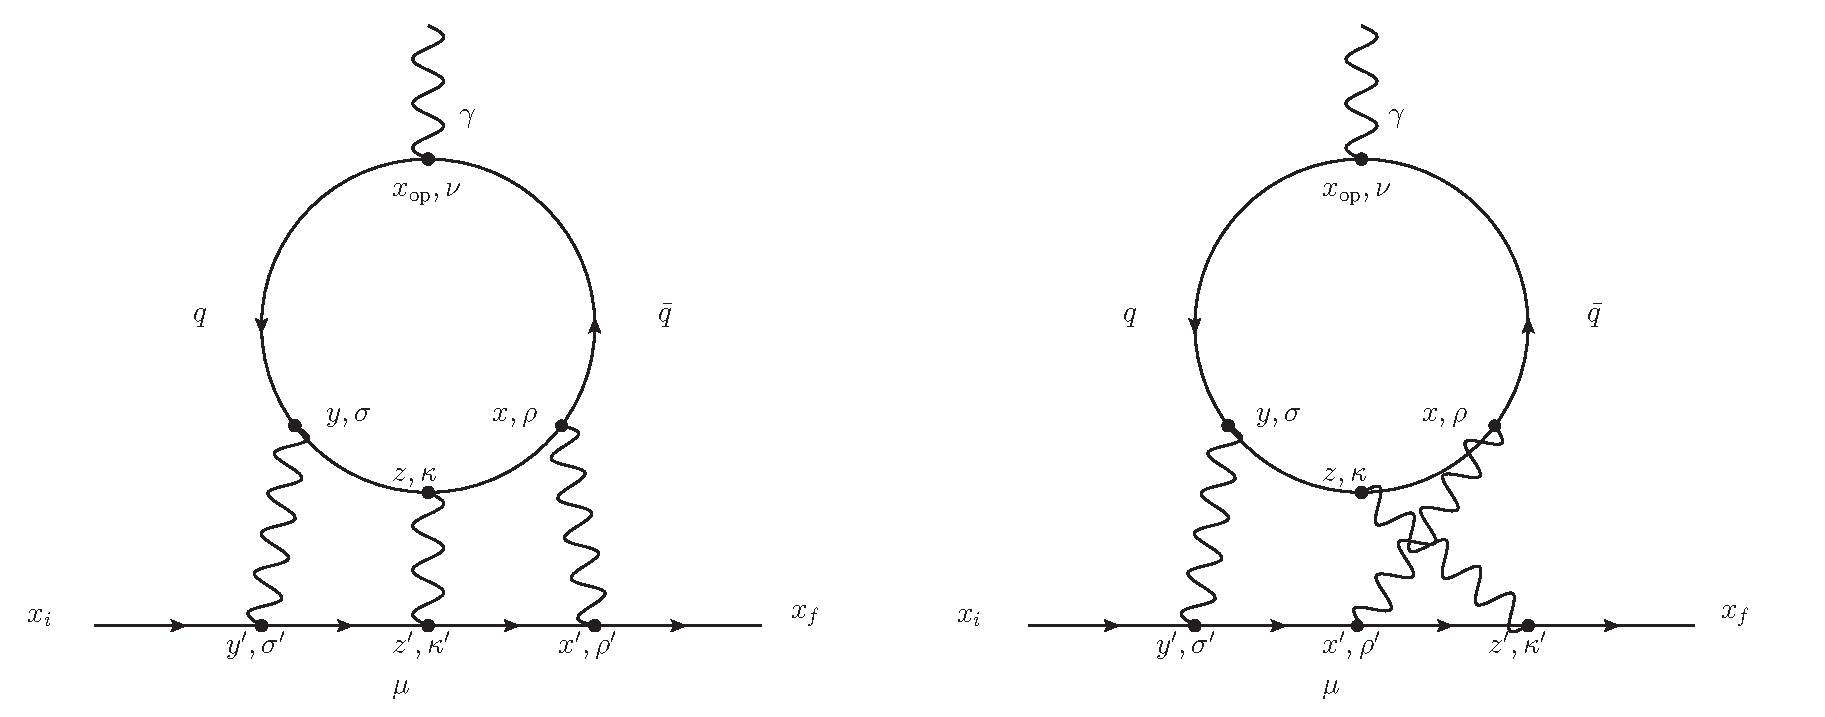
\includegraphics[scale=0.45]{hlblnotated.eps}%
    \caption{Feynman diagrams depicting hadronic light-by-light contributions to the muon anomalous magnetic moment. Above are two of the 6 possible contributions, each a unique permutation of the internal photon propagator with the external muon line.}%
    \label{hadlbl}%
\end{figure}


It is clear from Figure \ref{hadlbl} that these contributions begin at the $\mathcal{O}(\alpha^3)$ order. They involve a fermion loop with four photons attached to it\cite{lehnerg2}. In our case, we specialise the case to a $q-\bar{q}$ loop. The identical nature of the photons means there are $3!=6$ different configurations for the internal photons (labelled by Lorentz indices $\sigma, \kappa, \rho$), so one would expect six amplitudes contributing to $a_\mu^\mathrm{HLbL}$ at $\mathcal{O}(\alpha^3)$ order.

In order to express $a_\mu^\mathrm{HLbL}$ in terms that can be computed on the lattice, we begin from the field theoretic point of view and tailor it to yield quantites that can be evaluated using lattice QCD. Following \cite{zee}, we start with the Dirac equation for a fermion field, $\psi$,

\begin{equation}
(i\slashed{\partial} -m)\psi=0,
\label{dirac eq}
\end{equation}

\noindent where $\slashed{\partial} \equiv \gamma^\mu\partial_\mu$ and $\gamma^\mu$ are the four gamma matrices. The contraction of Lorentz indices, $\mu$ is also assumed. In momentum space, we can decompose $\psi$ into different modes,

\begin{equation}
\psi(x) = \int \frac{d^4p}{(2\pi)^4} \, u(p) e^{ip\cdot x},
\end{equation}

\noindent where $u(p)$ are the plane wave solutions\cite{tong}. In momentum space, Equation \ref{dirac eq} then becomes

\begin{equation}
(\slashed{p} - m)u(p) = 0.
\label{dirac eq in momentum space}
\end{equation}

\noindent If we multiply on the left hand side of Equation \ref{dirac eq in momentum space} with a factor of $\bar{u}(p)\gamma^\mu$ and add to it the complex conjugate, we obtain the Gordon decomposition:

\begin{equation}
\begin{split}
\bar{u}(p')(\gamma^\mu(\slashed{p}-m) + (\slashed{p'}-m)\gamma^\mu)u(p) &= 0,\\
\bar{u}(p')(\gamma^\mu\slashed{p} + \slashed{p'}\gamma^\mu- 2m\gamma^\mu)u(p) &= 0,\\
\frac{1}{2m}\bar{u}(p')(\gamma^\mu\gamma^\nu p_\nu + \gamma^\nu p'_\nu\gamma^\mu)u(p) &= \bar{u}(p')\gamma^\mu u(p),\\
\frac{1}{2m}\bar{u}(p')( (\eta^{\mu\nu} - iS^{\mu\nu})p_\nu + (\eta^{\mu\nu} + iS^{\mu\nu}) p'_\nu)u(p) &= \bar{u}(p')\gamma^\mu u(p),\\
\bar{u}(p')\left( \frac{\eta^{\mu\nu}(p_\nu + p'_\nu)}{2m} + \frac{iS^{\mu\nu}(p'_\nu - p_\nu)}{2m} \right)u(p) &= \bar{u}(p')\gamma^\mu u(p),\\
\bar{u}(p')\left( \frac{(p + p')^\mu}{2m} + \frac{iS^{\mu\nu}(p'_\nu - p_\nu)}{2m} \right)u(p) &= \bar{u}(p')\gamma^\mu u(p),
\end{split}
\label{gordon decomposition}
\end{equation}

\noindent where $S^{\mu\nu} = \frac{1}{2}[\gamma^\mu,\gamma^\nu]$. With foresight\cite{zee}, we note that the second term on the l.h.s involves the spin of the fermion due to the presence of the gamma matrices, and it is this term that gives the magnetic moment.

Next, we consider the matrix element of the electromagnetic current. Sandwiched between the muon initial and final state of momentum and spin $p,s$ and $p',s'$ respectively, Lorentz invariance and current conservation gives us

\begin{equation}
\braket{p',s'|J^\mu(0)|p,s} = -e\bar{u}(p',s')\left( \gamma^\mu F_1(q^2) + \frac{iS^{\mu\nu}q_\nu}{2m}F_2(q^2) \right)u(p,s).
\end{equation}

\noindent where $q = p'-p$ is the momentum transfer and $F_i(q^2)$ with $i=1,2$ are called form factors. Now, we can apply the Gordon decomposition derived in Equation \ref{gordon decomposition} and obtain

\begin{equation}
\begin{split}
\braket{p',s'|J^\mu(0)|p,s} = -e\bar{u}(p',s')\left( \left( \frac{(p+p')^\mu }{2m} + \frac{iS^{\mu\nu}q_\nu}{2m} \right) F_1(q^2)\right.&\\
\left. + \frac{iS^{\mu\nu}q_\nu}{2m}F_2(q^2) \right)u(p,s).&
\end{split}
\label{em current}
\end{equation}

For small $q^2$, we can expand the form factors. Considering only terms up to linear order in $q$,

\begin{equation}
\begin{split}
\braket{p',s'|J^\mu(0)|p,s} = -e\bar{u}(p',s')\left( \left( \frac{(p+p')^\mu }{2m} + \frac{iS^{\mu\nu}q_\nu}{2m} \right) (F_1(0) \right.&\\
\left.  + q^2F'_1(0) + \mathcal{O}(q^4)) + \frac{iS^{\mu\nu}q_\nu}{2m}(F_2(0) + q^2F'_2(0) + \mathcal{O}(q^4)) \right)u(p,s).&
\end{split}
\end{equation}
\begin{equation}
\begin{split}
\braket{p',s'|J^\mu(0)|p,s} = -e\bar{u}(p',s')\left( \frac{(p+p')^\mu }{2m} F_1(0) + \frac{iS^{\mu\nu}q_\nu}{2m}(F_1(0)+F_2(0)) \right)u(p,s).&
\end{split}
\label{em current with amu encoded}
\end{equation}

We can identify the first term in the brackets on the r.h.s as the electric charge\cite{zee} of the muon, which can be experimentally observed. The interesting piece contains the magnetic moment of the muon, quantified as $F_1(0) + F_2(0)$. Since $F_1(0)$, by definition, is set to unity, any shifts in the leptonic magnetic moment, for example, due to HLbL scattering processes, will be captured by $F_2(0)$. Thus, we find that \cite{blum}

\begin{equation}
a_\mu = F_2(0).
\end{equation}

On the lattice, we work with the l.h.s of Equation \ref{em current with amu encoded}. This establishes a method of comparison between theoretical (l.h.s) and experimentally measured (r.h.s) values. This involves evaluating Euclidean space Green's functions, which contains a muon source and sink with definite incoming and outgoing momenta. According to Blum \textit{et al.}\cite{blum}, this is chosen as $\vec{Q}/2$ and $-\vec{Q}/2$ respectively, where we remain notationally consistent with $\vec{Q}$ denoting the Euclidean momentum. 

In Euclidean space, the l.h.s of Equation \ref{em current with amu encoded} becomes

\begin{equation}
\langle \mu(x_f) J^\nu(x_\mathrm{op}) \bar{\mu}(x_i)\rangle,
\end{equation}

\noindent which is to be interpreted as a muon being created at the source, denoted by $\vec{x}_i$, where it interacts with the photon and is annihilated at the sink, denoted by $\vec{x}_f$. This quantity is equal to the product of electric charge and the amplitude of the process, $-e\mathcal{M}(\vec{x}_i,\vec{x}_\mathrm{op},\vec{x}_f)$, which is defined as

\begin{equation}
\mathcal{M}_\nu(\vec{Q}) = \lim_{\substack{t_i\rightarrow -\infty\\t_f \rightarrow \infty}} e^{E(t_f-t_i)} \sum_{\vec{x}_i,\vec{x}_f}e^{-i\frac{\vec{Q}}{2}(\vec{x_i}+\vec{x_f})}e^{i\vec{Q}\cdot\vec{x}_{op}} \mathcal{M}_\nu(x_i,x_\mathrm{op}, x_f).
\label{amplitude on the lattice}
\end{equation}

\noindent where $E=\sqrt{m_\mu^2+|\vec{Q}/2|^2}$. We now have an equation for computing the total amplitude of an electromagnetic interaction on the lattice. In Equation \ref{amplitude on the lattice}, we sum over all local amplitudes $\mathcal{M}_\nu(x_i,x_{\mathrm{op}},x_f)$ due to every possible sink-source combination on the lattice volume. We note that the exponential factor $e^{-i\vec{Q}/2(\vec{x}_f-\vec{x}_i)}$ was included to ensure that the total amplitude on the l.h.s is translation invariant. 

As mentioned in the opening paragraph of this section, there are $3!=6$ different Feynman diagrams to consider, each corresponding to different arrangement of the internal photons as illustrated in Figure \ref{hadlbl}. We can thus re-express the amplitude $\mathcal{M}_\nu(x_i,x_\mathrm{op},x_f)$ as the sum of these six graphs' amplitude. This can be done by summing over the Feynman amplitudes with different spacetime configurations as

\begin{equation}
\mathcal{M}_\nu(x_i,x_\mathrm{op},x_f) = \sum_{x,y,z} \mathcal{F}_\nu(x,y,z,x_\mathrm{op},x_i,x_f),
\label{Feynman amplitude}
\end{equation} 

\noindent where $x,y,z$ are spacetime points as seen in Figure \ref{hadlbl}. These specific Feynman amplitudes can be deduced from Feynman rules, easily compiled in texts such as \cite{tong}. Schematically, we have 

\begin{equation}
\begin{split}
\mathcal{F}_\nu(x,y,z,x_\mathrm{op},x_i,x_f) \equiv \quad &\mathrm{``all \, possible} \,  \mathrm{internal \, quark \, lines"} \\
\times &\mathrm{``internal \, photon \, propagators"}\\
\times &\mathrm{``permutations \, of \, internal \, muon \, propogators"}.
\end{split}
\end{equation}

\noindent Formally, it is written as

\begin{equation}
\begin{split}
\mathcal{F}_\nu &(x,y,z,x_\mathrm{op}, x_i, x_f) = -(-ie)^3 \\
& \times \sum_{q\in \{u,d,s\}}(ie_q)^4 \left\langle \, \mathrm{Tr}[\gamma_\nu S_q(x_\mathrm{op},x) \gamma_\rho S_q(x,z) \gamma_\kappa S_q(z,y) \gamma_\sigma S_q(y,x_\mathrm{op})]_\mathrm{QCD} \right\rangle \\
&\times \sum_{x',y',z'} G_{\rho\rho '}(x,x')G_{\kappa\kappa '} (z,z') G_{\sigma\sigma '}(y,y')\\
&\times \left( S_\mu(x_f,x') \gamma_{\rho '} S_\mu(x',z') \gamma_{\kappa '} S_\mu(z',y') \gamma_{\sigma '} S_\mu(y',x_i) + \mathrm{5 \, other \, permutations} \right),
\end{split}
\label{Feynman amplitude full}
\end{equation}

\noindent where $S_\mu$ are the muon propagators, $G_{\alpha \alpha '}$ with $\alpha \in \{\rho,\kappa,\sigma \}$ are the photon propagators and $S_q$ are the internal quark propagators. The cubic factor of $-ie$ at the front comes from the coupling between the internal photon propagator with the muon line. The QCD subscript of the trace represents an average over all QCD gauge configutations. This is responsible for providing the background fields in which the quark propagators can be computed on. The $-e$ and $e_q$ are the muon and quark electric charge respectively, where $e_q = 2e/3 \, \, \mathrm{or} -e/3$ depending on the quark in context.  

During the time of writing this paper \cite{blum} in 2015, it is computationally expensive to evaluate $\mathcal{F}_\nu$ directly on the lattice. Below, we explore two stochastic methods proposed by Blum \textit{et al.} to circumvent the problem of computing resources.

\subsubsection{Exact Photon Propogators}

To introduce random sampling using Equation \ref{Feynman amplitude full} directly is computationaly expensive, even with a single QCD configuration. To that end, we express the total amplitude $\mathcal{M}_\nu(\vec{Q})$ as an explicit sum of three additional spacetime vertices, $x,y,z$ at which the internal photon line couples to the quark line 

\begin{equation}
\mathcal{M}_\nu(\vec{Q}) = e^{i\vec{Q}\cdot\vec{x}_\mathrm{op}} \sum_{x,y,z} \mathcal{F}_\nu(\vec{Q},x,y,z,x_\mathrm{op}),
\label{total amplitude with spacetime}
\end{equation}

\noindent where we note that the Feynman amplitude now depends on the Euclidean momentum, $\vec{Q}$, as well. As before, the factor of $e^{i\vec{Q}\cdot\vec{x}_\mathrm{op}}$ is present to maintain translation invariance of $\mathcal{M}_\nu(\vec{Q})$. It is also independent of the time of propogation, $t_\mathrm{op}$. We can identify this modified Feynman amplitude as 

\begin{equation}
\mathcal{F}_\nu(\vec{Q},x,y,z,x_\mathrm{op}) = \lim_{\substack{t_i\rightarrow -\infty\\t_f \rightarrow \infty}} e^{E(t_f-t_i)} \sum_{\vec{x}_i,\vec{x}_f}e^{-i\frac{\vec{Q}}{2}(\vec{x_i}+\vec{x_f})} \mathcal{F}_\nu(x,y,z,x_i,x_\mathrm{op}, x_f)
\end{equation}

\noindent from Equation \ref{amplitude on the lattice}. Blum \textit{et al.} then make an arbitrary choice and let $\vec{Q} = \frac{2\pi}{L}\vec{z}$, where $L$ is the spatial extent of the lattice. Since the muons are fermions, their propogators, $S_\mu$ are evaluated in the z-direction with anti-periodic boundary conditions, that is,

\begin{equation}
\psi(P) = -\psi(0),
\end{equation}

\noindent where $P$ denotes the period. This is to ensure that trace of an operator remains consistent in the path integral formalism for fermions\cite{antiperiodic}. 

We will now exploit the spacetime translation covariance of $F_\nu(\vec{Q},x,y,z,x_\mathrm{op})$. Starting with Equation \ref{total amplitude with spacetime}, we rewrite the arguments that describe the spacetime positions relative to the quark loop. This involves shifting the position variables of $F_\nu$ by the average, $w=\frac{x+y}{2}$. In Equation \ref{total amplitude with spacetime}, this translates to

\begin{equation}
\begin{split}
\mathcal{M}_\nu(\vec{Q}) &= \sum_{x,y,z} e^{i\vec{Q}(\vec{x}_\mathrm{op}-\vec{w})} \mathcal{F}_\nu(\vec{Q},x-w,y-w,z-w,x_\mathrm{op}-w), \\
&= \sum_{x,y,z} e^{i\vec{Q}(\vec{x}_\mathrm{op}-\vec{w})} \mathcal{F}_\nu(\vec{Q},\frac{x-y}{2},-\frac{x-y}{2},z-w,x_\mathrm{op}-w),\\
&= \sum_r\left(\sum_{\tilde{z},\tilde{x}_\mathrm{op}} e^{i\vec{Q}\cdot\tilde{\vec{x}}_\mathrm{op}} \mathcal{F}_\nu(\vec{Q},\frac{r}{2},-\frac{r}{2},\tilde{z},\tilde{x}_\mathrm{op})\right),
\end{split}
\label{amplitude by average}
\end{equation}

\noindent where we have introduced a notational shorthnd for the shifted variables, $\tilde{z}=z-w$ and $\tilde{x}_\mathrm{op}=x_\mathrm{op}-w$. In going from the second line to the third, we note that summing over $x$ and $y$ after the shift by the average is equivalent to summing over the $r=x-y$ values, so we can replace the two spacetime summations with $r$, which is performed only after we have completely summed over the shifted $z$-direction and the propogation coordinates.

Equation \ref{amplitude by average} gives a natural strategy to evaluate on the lattice. First, we make a random choice to $w$ somewhere within the spacetime volume. To ensure that $t_f-t_i$ is large in accordance to Equation \ref{amplitude on the lattice}, corresponding to the limit $t\rightarrow \pm \infty$, we choose, in context of the lattice

\begin{equation}
\begin{split}
t_i &= (x_\mathrm{op})_0 -\frac{T}{4},\\
t_f &= (x_\mathrm{op})_0 +\frac{T}{4},
\end{split}
\end{equation}

\noindent where $T$ is the temporal extent of the lattice volume. The coordinate $r$ can be used to introduce stochastic effects. We can employ $r/2$ and $-r/2$ as source locations of two propogators whose sinks are joined at the shifted positions $\tilde{z}$ and $\tilde{x}_\mathrm{op}$. When summed over $w$ and $r$ and averaged over the QCD gauge configurations, Equation \ref{amplitude by average} gives the muon-current 3-point function. 

This method has an advantage that in the limit of infinite volume on the lattice, we only have finite statistical noise.


\subsubsection{Obtaining $q^2=0$ in Finite Volume}

In this method, we work with the matrix element of the electromagnetic current in Equation \ref{em current}. For convenience, we restate it here:

\begin{equation}
\begin{split}
\braket{p',s'|J^\mu(0)|p,s} = \bar{u}(p',s')\left( \left( \frac{(p+p')^\mu }{2m} + \frac{iS^{\mu\nu}q_\nu}{2m} \right) F_1(q^2)\right.&\\
\left. + \frac{iS^{\mu\nu}q_\nu}{2m}F_2(q^2) \right)u(p,s).&
\end{split}
\label{em current (repeated)}
\end{equation}

This contains the form factor $F_2(q^2)$ multiplied with components of momentum transfer $q_\rho$. Speacialising in Euclidean momentum, $F_2(Q^2)$ can be obtained from lattice calculation when $Q_\rho \neq 0$ such that $a_\mu = F_2(0)$ can be determined in the limit of $Q_\rho\rightarrow 0$. However, this is difficult to perform on the lattice since the smallest non-zero momentum component is $\frac{2\pi}{L}$, where $L$ is the spatial extent of the lattice. Thus, in the limit of $Q_\rho \rightarrow 0$ we require $L\rightarrow\infty$, which corresponds to the infinite volume limit. A solution to the problem of finite computation resource is to define a spatial moment for the Feynman amplitude, which in turn determines the matrix element of $J_\nu(0)$, as we will see below.

We begin with Equation \ref{amplitude by average}. For convenience, we drop the tilde on the shifted variables

\begin{equation}
\mathcal{M}_\nu(\vec{Q})= \sum_r\left(\sum_{z,x_\mathrm{op}} e^{i\vec{Q}\cdot\vec{x}_\mathrm{op}} \mathcal{F}^c_\nu(\vec{Q},\frac{r}{2},-\frac{r}{2},z,x_\mathrm{op})\right),
\label{amplitude by average repeated}
\end{equation}

\noindent where we have also added a superscript $c$ in foresight of working towards the electromagnetic current. $\mathcal{F}^c_\nu$ has the same dependence on $x_\mathrm{op}$ as $J_\nu$, which means it also obeys the same Ward identity. This can be expressed as 

\begin{equation}
\Delta_{\mathrm{(op)}\nu}F^c_\nu(\vec{Q},x,y,z,x_\mathrm{op})=0,
\end{equation}

\noindent where the contraction of the Lorentz index $\nu$ is implied. We also remind ourselves that in Euclidean space, the covariant and contravariant indices bear no distinction. Here, $\Delta_{\mathrm{(op)}\nu}$ is the backwards lattice measure of change, defined as 

\begin{equation}
\Delta_xf(x) = f(x) - f(x-a),
\end{equation}

\noindent which we recall is the difference in values of $f$ between neighbouring lattice sites, where $a$ is the lattice spacing. 

Now, the key step is to replace $e^{i\vec{Q}\cdot\vec{x}_\mathrm{op}}$ with $e^{i\vec{Q}\cdot\vec{x}_\mathrm{op}}-1$, giving

\begin{equation}
\mathcal{M}_\nu(\vec{Q})= \sum_r\left(\sum_{z,x_\mathrm{op}} \mathcal{F}^c_\nu(\vec{Q},\frac{r}{2},-\frac{r}{2},z,x_\mathrm{op})(e^{i\vec{Q}\cdot\vec{x}_\mathrm{op}}-1)\right).
\label{amplitude by average -1}
\end{equation}

This is perfectly consistent with Equation \ref{amplitude by average repeated} since the factor of -1 introduced will vanish due to the Ward identity. This is demonstrated below, with arguments suppressed,

\begin{equation}
\begin{split}
\sum_{r,z,x_\mathrm{op}}\Delta_\nu F_\nu &= 0,\\
\sum_{r,z,x_\mathrm{op}}x\Delta_\nu F_\nu &= 0,\\
\Rightarrow\sum_{r,z,x_\mathrm{op}}x_\rho\Delta_\nu F_\nu &= \sum_{r,z,x_\mathrm{op}} \Delta_\nu (x_\rho F_\nu) - \sum_{r,z,x_\mathrm{op}}\delta_{\rho\nu}F_\nu,\\
0&= -\sum_{r,z,x_\mathrm{op}}F_\rho,
\end{split}
\end{equation}

\noindent which is as we claimed in the paragraph above, assuming that the surface term $\Delta_\nu(x_\rho F_\nu)$ goes to zero sufficiently fast upon summation.

Now, we can expand Equation \ref{amplitude by average -1} in $\vec{Q}$ from both the exponential and the amplitude. Once again, we suppress the irrelevant arguments to prevent a cluttering of notation. To linear order in small $\vec{Q}$, 

\begin{equation}
\begin{split}
\mathcal{M}_\nu(\vec{Q})&= \sum_r\left(\sum_{z,x_\mathrm{op}} (\mathcal{F}^c_\nu(0)+ Q_j\frac{\partial\mathcal{F}^c_\nu}{\partial Q_j}\bigg\vert_{Q=0}+ \mathcal{O}(Q^2))(1+iQ_k\cdot x_{\mathrm{op},k} + \mathcal{O}(Q^2)-1)\right),\\
&=\sum_r\left(\sum_{z,x_\mathrm{op}} (iQ_k\cdot x_{\mathrm{op},k}\mathcal{F}^c_\nu(0)+ \mathcal{O}(Q^2)\right),\\
\end{split}
\end{equation}

\noindent taking the derivative of $\mathcal{\vec{Q}}$ and evaluating it at $\vec{Q}=0$,

\begin{equation}
\begin{split}
\frac{\partial}{\partial Q_j}\mathcal{M}_\nu(0) &= \sum_r\left(\sum_{z,x_\mathrm{op}} (i\delta_{jk}\cdot x_{\mathrm{op},k}\mathcal{F}^c_\nu(0)+ \mathcal{O}(Q)\right)\bigg\vert_{Q=0},\\
&= i\sum_r\sum_{z,x_\mathrm{op}} \mathcal{F}^c_\nu(0) \, x_{\mathrm{op},j},\\
\end{split}
\label{moment hlbl}
\end{equation}

This equation is derived in an infinite spacetime volume, captured by the fact that $\mathcal{M}_\nu(\vec{Q})$ has neither spacetime dependence nor arguments in $x_\mathrm{op}$. However, since $\mathcal{F}^c_\nu$ is a function of $r$ and $-r$, the average, by symmetry, is location at the origin. which means that $F_\nu^c$ deceases exponenetially with increasing $|x_\mathrm{op}|$. In terms of lattice QCD, this implies that the summation can be carried out in a large but nonetheless finite volume with exponentially small corrections.

We want to make contact with the form factor, $F_2(0)$ in Equation \ref{em current (repeated)} since this is where we can compute $a_\mu$. We know that the l.h.s of Equation \ref{em current (repeated)} is equal to $-e\mathcal{M}_\nu$. In Euclidean space,

\begin{equation}
\begin{split}
-e\mathcal{M}_\nu(Q)= -e\bar{u}(Q',s')\left( \left( \frac{(Q+Q')^\mu }{2m} - \frac{iS^{\mu\nu}Q_\mu}{2m} \right) F_1(Q^2) - \frac{iS^{\mu\nu}Q_\mu}{2m}F_2(Q^2) \right)u(Q,s),
\end{split}
\label{amplitude - emcurrent element}
\end{equation}

\noindent where we picked up a minus sign for the $Q_\mu$ terms due to the relabelling $\mu\rightarrow\nu$ and $\nu\rightarrow\mu$.

In the limit of $t_i \rightarrow -\infty$ and $t_f \rightarrow \infty$, $u(Q,s$ and $\bar{u}(Q',s')$ become energy eigenstates of the free theory Hamiltonian \cite{tong}. This allow us to write

\begin{equation}
u(Q) = \frac{-i\slashed{Q}^-+m_\mu}{2E} \quad \mathrm{and} \quad \bar{u}(Q') = \frac{-i\slashed{Q'}^++m_\mu}{2E},
\end{equation}

\noindent where $Q^\pm = (iE,\pm \vec{Q}/2)$ and $E=\sqrt{m_\mu^2 + |\vec{Q}/2|^2}$. Equation \ref{amplitude - emcurrent element} now takes the following form

\begin{equation}
\mathcal{M}_\nu(Q) = -\left(\frac{-i\slashed{Q'}^++m_\mu}{2E}\right)\left( \frac{iS^{\mu\nu}Q_\mu}{2m}F_2(Q^2) \right)\left(\frac{-i\slashed{Q}^-+m_\mu}{2E}\right),
\label{amplitude - emcurrent element f2 only}
\end{equation}

\noindent where we have omitted the $F_1(Q^2)$ term since we are only interested in contributions to $a_\mu$.

To make contact with Equation \ref{moment hlbl}, we expand the r.h.s of Equation \ref{amplitude - emcurrent element f2 only} to linear order in the limit of small momentum transfer, $Q=0$. Then, take the derivative with respect to $Q_i$ and then evaluate the expression at $Q=0$. For the moment, define $f^{-}(Q) = (-i\slashed Q^{-} + m_\mu)/2E$ and similarly for the primed positive energy solution as the expansion in the limit of small Q,

\begin{equation}
\begin{split}
\frac{\partial}{\partial Q_i} \mathcal{M}_\nu(Q)\bigg\vert_{Q=0} &\approx \frac{\partial}{\partial Q_i}\left[-f'^+(Q)\left( \frac{iS^{\mu\nu}Q_\mu}{2m}(F_2(0) \right.\right. \\
& \left. \left. + Q^2\frac{\partial^2}{\partial Q^2}F_2(Q^2)) + \mathcal{O}(Q^4) \right)f^-(Q) \right]\bigg\vert_{Q=0},\\
&= -f'^+(Q)\left( \frac{iS^{\mu\nu}}{2m}\delta_{i\mu}F_2(0)\right)f^-(Q)\bigg\vert_{Q=0} + \cdots,\\
\end{split}
\label{moment - f2}
\end{equation}

\noindent where the $\cdots$ denote terms including derivatives of $f'^+$ and $f^-$, which will vanish when $Q=0$ due to the $Q_\nu$ coupled to $F_2(Q^2)$. Now if we sandwich Equation \ref{moment - f2} with zero momentum positive energy eigenstates, $\bar{u}(s')$ and $u(s)$, on the r.h.s we get the term

\begin{equation}
\begin{split}
-\bar{u}(s)f'^+(Q)\left( \frac{iS^{i\nu}}{2m}F_2(0)\right)f^-(Q)\bigg\vert_{Q=0} u(s)
\end{split}
\end{equation}

Now, if we write out explicitly the expansions $f'^+(Q)$ and $f^-(Q)$, we have

\begin{equation}
\begin{split}
\frac{1}{E} &= \frac{1}{\sqrt{m_\mu^2 + |\frac{Q}{2}|^2}},\\
\frac{1}{E} &\approx \frac{1}{m_\mu} -\frac{1}{2!}\frac{Q^2}{m_\mu^3} + \mathcal{O}(Q^4),\\
\Rightarrow\frac{-i\slashed{Q'}^++m_\mu}{2E} &= (-i(\gamma^0(iE) + \gamma^kQ_k) +m_\mu)\frac{1}{2}\left(\frac{1}{m_\mu} -\frac{1}{2!}\frac{Q^2}{m_\mu^3} + \mathcal{O}(Q^4)\right),\\
&= (\gamma^0E - i\gamma^kQ_k +m_\mu)\frac{1}{2}\left(\frac{1}{m_\mu} -\frac{1}{2!}\frac{Q^2}{m_\mu^3} + \mathcal{O}(Q^4)\right),\\
\bar{u}(s')\frac{-i\slashed{Q'}^++m_\mu}{2E} &= \bar{u}(s')(\gamma^0E - (i+1)\gamma^kQ_k +m_\mu)\frac{1}{2}\left(\frac{1}{m_\mu} -\frac{1}{2!}\frac{Q^2}{m_\mu^3} + \mathcal{O}(Q^4)\right),\\
&= \bar{u}(s')(2m_\mu - (i+1)\gamma^kQ_k)\frac{1}{2}\left(\frac{1}{m_\mu} -\frac{1}{2!}\frac{Q^2}{m_\mu^3} + \mathcal{O}(Q^4)\right),\\
\Rightarrow \bar{u}(s')f'^+(Q)&= \bar{u}(s')+\mathcal{O}(Q),\\
\end{split}
\end{equation}

\noindent where in going to the penultimate line, we used Equation \ref{dirac eq in momentum space}. We note the $\mathcal{O}(Q)$ terms will vanish since the final expression is evaluated at $Q=0$. We get a similar term for $f^-(Q)u(s)$:

\begin{equation}
u(s)f'^-(Q)= u(s)+\mathcal{O}(Q).
\end{equation}


%Now consider the Dirac equation,
%
%\begin{equation}
%(i\slashed\partial-m)\psi=0.
%\end{equation}
%
%\noindent Rewriting it in terms of the plane wave solutions, we get a relation between the momentum and the muon mass,
%
%\begin{equation}
%\begin{split}
%\mathrm{Let} \, \psi(x) = u(p)e^{-ip\cdot x}
%\end{split}
%\end{equation}


%In Euclidean space, we perform a Wick rotation, followed by a Fourier transform of $\psi$,
%
%\begin{equation}
%\begin{split}
%t &\rightarrow it,\\
%x^\mu & \rightarrow \tilde{x}^\mu = (it,\vec{x}),\\
%\psi(x) &= i\int \frac{d^4x}{(2\pi)^4} \, u(Q) e^{iQ\cdot x},
%\end{split}
%\end{equation}
%
%\begin{equation}
%\begin{split}
%\Rightarrow (i\slashed\partial-m)\,i\int\frac{d^4x}{(2\pi)^4} \, u(Q) e^{iQ\cdot \tilde{x}}&=0,\\
%(i\slashed{\tilde{Q}}+m)u(Q)&=0, \quad \mathrm{with} \, \tilde{Q}=(iE,\vec{Q}),\\
%(i\gamma^0(iE) + i\gamma^jQ^j +m)u(Q)&=0,\\
%\Rightarrow \gamma^0Eu(Q) &= i\gamma^jQ^ju(Q) +mu(Q).
%\end{split}
%\end{equation}

Finally, we can put all the terms together and evaluate at $Q=0$, giving us

\begin{equation}
\bar{u}(s')\frac{\partial}{\partial Q_i} \mathcal{M}_\nu(Q)\bigg\vert_{Q=0}u(s) = -\bar{u}(s')\left( \frac{iS^{i\nu}}{2m}F_2(0)\right)u(s)
\label{moment - f2 final}
\end{equation}

Specialising in the spatial component, $\nu=j$, we introduce the expression for $\mathcal{M}_\nu$ into Equation \ref{moment - f2 final},

\begin{equation}
i\bar{u}(s')\sum_r\sum_{z,x_\mathrm{op}} \mathcal{F}^c_j(0) \, x_{\mathrm{op},i}u(s) = -\bar{u}(s')\left( \frac{iS^{ij}}{2m}F_2(0)\right)u(s).
\label{feynman amplitude - f2}
\end{equation}

Multiplying Equation \ref{feynman amplitude - f2} by $\frac{1}{2}\epsilon_{ijk}$, we get a vector equation

\begin{equation}
\begin{split}
\frac{1}{2} \bar{u}(s')\sum_r\sum_{z,x_\mathrm{op}} i\mathcal{F}^c_j(0) \, \epsilon_{ijk} x_{\mathrm{op},i}u(s) &= -\frac{1}{2}\bar{u}(s')\left( \epsilon_{ijk}\frac{iS^{ij}}{2m}F_2(0)\right)u(s),\\
 &= \frac{F_2(0)}{2m}\bar{u}(s')\Sigma_ku(s),\\
\frac{1}{2} \sum_{r,z,x_\mathrm{op}} \vec{x}_{\mathrm{op}} \times i\bar{u}(s')\vec{\mathcal{F}}^c(0)u(s) \, \epsilon_{ijk}  &= \frac{F_2(0)}{2m}\bar{u}(s')\vec{\Sigma} u(s),
\end{split}
\label{feynman amplitude - f2 final}
\end{equation}

\noindent where $\Sigma_k = \frac{1}{4i}\epsilon_{ijk}[\gamma^i,\gamma^j]$. We also note that the term $i\mathcal{F}^c(0)$ is equivalent to the quantum mechanical current. Indeed, the l.h.s of Equation \ref{feynman amplitude - f2 final} has the same form as a magnetic moment, $\mu$, produced by a static (time-independent), localised current, $J(r)$. In the continuum form, 

\begin{equation}
\vec{\mu} = \frac{1}{2}\int d^3r \, \vec{r} \times \vec{J}(\vec{r}),
\label{magnetic moment analogy}
\end{equation}

\noindent where $\vec{\mu}$ is the magnetic moment vector, $\vec{r}$ is the position vector and $\vec{J}(\vec{r})$ is the classical electric current. For the details regarding the relation between Equation \ref{magnetic moment analogy} and \ref{feynman amplitude - f2 final}, we refer to \cite{blum}.

The $\vec{x}_{\mathrm{op}} \times i\bar{u}(s')\vec{\mathcal{F}}^c(0)u(s)$ is the sought after expression, known as the (spatial) moment of the Feynman amplitude. When we trace back the derivation, we note that this expression originates from the matrix element of the electromagnetic current, for example see Equation \ref{em current (repeated)} and \ref{moment hlbl}. As mentioned in the paragraph below Equation \ref{moment hlbl}, the presence of the Feynman amplitude $\mathcal{F}_\nu$ allows us to study the HLbL contributions at finite, albeit large volume on the lattice with small corrections, thereby circumventing the problem of taking $L\rightarrow \infty$. 

Since the HLbL scattering contribution cannot be related to experimental data, alternative approaches to compute $a_\mu^\mathrm{HLbL}$ are model-dependent\cite{vainshtein}. Usually, they depend on theoretical parameters such as the smallness of chiral symmetry breaking or the large number of colour charges, $N_c$\cite{vainshtein}. For example, Melnikov and Vainshtein in 2004 considered contributions parametrised by $N_c$, producing a value of $a_\mu^\mathrm{HLbL} = (136\pm 25)\times 10^{-11}$, where the uncertainty is subjective to estimations of the pseudoscalar and pseudovector exchanges\cite{vainshtein}. For completeness, the model-independent HLbL contribution introduced by Blum \textit{et al.} in 2015 gives

\begin{equation}
a_\mu^\mathrm{HLbL} = (132.1 \pm 6.8) \times 10^{-11}\text{\cite{blum}}.
\end{equation}

\section{Conclusion}

The anomalous muon magnetic moment, $a_\mu$, is defined as the deviation from the Dirac moment\cite{zee}. This effect is due to radiative and higher order loop corrections. As such, the anomalous muon magnetic moment serves as an excellent low energy probe for new physics\cite{millerg2}, which appears as a discrepancy between the experimentally measured $a_\mu$ to that predicted by the Standard Model. The measurements made at the Brookhaven National Laboratory in the course of 1999 to 2001 yielded an experimental value of \cite{millerg2}

\begin{equation}
a_\mu^{\mathrm{E821}} = 11 659 208.0(5.4)(3.3) \times 10^{-10},
\end{equation}

\noindent where the current experiment, E989, at Fermilab promises to increase the precision of the reuslt by four-fold\cite{fermilab}.

The theoretical predictions must match in terms of precision with the ever-improving experimental setups. Recent progress by Aoyama \textit{et al.} in \cite{aoyama} have computed QED contributions to $a_\mu^\mathrm{SM}$ up to the tenth order and Gnendiger \textit{et al.}\cite{gnendiger} have completed the EW contributions up to two loops. Together, the QED and EW contributions yield

\begin{equation}
\begin{split}
a^{\mathrm{QED}}_\mu&= 116 584 718 951 (80) \times 10^{-14}\text{\cite{aoyama}} \quad (2017),\\
a^{\mathrm{EW}}_\mu &= (153.6\pm 1.0) \times 10^{-11}\text{\cite{gnendiger}} \quad (2017)
\end{split}
\end{equation}

\noindent where the uncertainty in QED contributions come from measurement of the Rydberg constant\cite{aoyama} and the EW contributions come from three-loop and hadronic contributions\cite{gnendiger}.

While the QED contributions are dominant in $a_\mu^\mathrm{SM}$, the main theoretical uncertainty originates from hadronic contributions. This literature review focusses on the two hadronic contributions - the hadronic vacuum polarisation and the hadronic light-by-light scattering processes - and the numerical techniques applied in lattice QCD to evaluate them.

The hadronic vacuum polsarisation makes its contribution to $a_\mu^\mathrm{had}$ via Equation \ref{ahvp}. The main challenge of evaluating Equation \ref{ahvp} on the lattice is due the need for large lattice dimensions at $\mathcal{O}(10\mathrm{fm})$, which is much too expensive for current computational resources. To this end, we explored two methods. The first is in switching the kernel function in Equation \ref{ahvp} into its time-momentum representation, $\tilde{K}(t;m_\mu)$. This gives us an explicit expression for the kernel function with an accuracy up to $\mathcal{O}(10^{-6})$. Another strategy to evaluate Equation \ref{ahvp} is to find an expression for the once subtracted vacuum polarisation function, $\hat{\Pi}(Q^2)$. The key insight proposed by Della Morte \textit{et al.} in \cite{dellamorte} is a hybrid strategy, where one can use the time moments as coefficients for the Pad\'e approximants to determine $\hat{\Pi}(Q^2)$ at low $Q^2$. The hadronic vacuum polarisation contribution to $a_\mu^\mathrm{had}$ due to the up, down, strange and charm quarks in time-momentum representation (TMR) and the hybrid strategy are summarised below\cite{dellamorte}


\begin{equation}
\begin{split}
a_\mu^\mathrm{HVP,TMR} &= (616.7 \pm 24.8 \pm 28.9) \times 10^{-10} ,\\
a_\mu^\mathrm{HVP,hybrid} &= (623.1 \pm 25.4 \pm 19.7) \times 10^{-10}, 
\end{split}
\end{equation}

\noindent where the first uncertainty is due to statistical error and the second is due to systematic error.

In principle,the contributions due to hadronic light-by-light scattering processes can be evaluated on the lattice using Equation \ref{Feynman amplitude full}. However, this is computationally expensive and alternative methods are used instead. The first explored in this review looks for a new method to introduce stochastic effects. This involves exploiting the translation covariance of the Feynman amplitude to shift its spacetime arguments by an average value that we can set. The second method involves deriving an expression for the amplitude moments and using it to compute the form factor, $F_2(0)$ on the lattice. The symmetry of the setup is such that the total amplitude receives most of the contribution at the origin of the lattice and becomes exponentially suppressed in the limit of infinite volume. Below, we quote the HLbL contribution to $a_\mu$ according to Blum\cite{blum}

\begin{equation}
a_\mu^\mathrm{HLbL} = (132.1 \pm 6.8) \times 10^{-11}\quad(2015),
\end{equation}

\noindent where the uncertainty quoted is due to statistical errors.

The discrepancy between the experimentally measured and theoretically predicted values of $a_\mu$ currently stands at 3.6$\sigma$\cite{lehnerg2}. It is clear from Aoyama's work\cite{aoyama} that while higher order corrections can reduce $a_\mu^\mathrm{exp} - a_\mu^\mathrm{SM}$, improving the precision of hadronic contributions to $a_\mu^\mathrm{SM}$ will provide the final say as to whether this discrepancy is an indication of new physics or otherwise. 



\newpage
\bibliographystyle{ieeetr} %the command ieeetr sorts citations in order  of appearance
\bibliography{muBib}




\end{document}

